\documentclass[lettersize,journal]{IEEEtran}
\usepackage{amsmath,amsfonts}
\usepackage{algorithm}
\usepackage{algorithmic}
\usepackage{array}
\usepackage[caption=false,font=normalsize,labelfont=sf,textfont=sf]{subfig}
\usepackage{textcomp}
\usepackage{stfloats}
\usepackage{url}
\usepackage{verbatim}
\usepackage{graphicx}
\usepackage{balance}
\usepackage{etoolbox}
\usepackage{amssymb}
\usepackage{bm}
\usepackage[colorlinks=true,citecolor=blue,linkcolor=blue,urlcolor=blue]{hyperref}

\newcommand{\figcaptiontight}{\par\vspace{-2.5mm}}

\hyphenation{op-tical net-works semi-conduc-tor IEEE-Xplore}

\begin{document}

\title{Bellman Conservation Law-based Crowd Flow Control via Passage Direction and Entrance-Rate Optimization in Metropolitan Tourism Hotspots: Scalability to 50,000 Pedestrians}

\author{Bingyu Wei, Rongyong Zhao, \textit{Member, IEEE}, Cuiling Li, Zhengyang Shi, Li Chen, Yuxin Cai, and Lingchen Han
\thanks{Bingyu Wei, Rongyong Zhao, Cuiling Li, Yuxin Cai, and Lingchen Han are with the CIMS Research Center, Tongji University, Shanghai 201804, China. (e-mail: \{weiby, zhaorongyong, licuiling, 2432091, 2432090\}@tongji.edu.cn). (\textit{Corresponding author: Rongyong Zhao}.)}
\thanks{Zhengyang Shi and Li Chen are with Huangpu Public Security Bureau, Shanghai, China. (e-mail: \{13817036566, kevin\_c2009\}@163.com).}}

% \markboth{Journal Name,~Vol.~XX, No.~X, Month~2026}%
% {Author: Channel Optimization for Crowd Management}

\maketitle

\begin{abstract}
Metropolitan tourism hotspots and major event venues are particularly vulnerable to crowd stampedes due to the high density and stochasticity of pedestrian flows. Yet existing control methods remain largely empirical and reactive, leaving the coupled effects of passage directions and time-phased admission rates insufficiently quantified. To address this academic issue,this paper develops a macroscopic crowd-control model based on the Bellman Conservation Law. Local admissible direction sets represent one-way, bidirectional, and closed passages, while anisotropic mobility tensors encode channel-guidance effects. Internal channel entrance-rate controls are added so that one policy specifies both passage directions and release rates. We then solve the mixed discrete-continuous problem with a Hierarchical Constrained Mixed-variable Black-box Optimization (HCMBO) algorithm. In a simplified scenic-platform scenario, the model reproduces multi-stage movement, channel guidance, and direction constraints. Under a weighted objective combining efficiency, safety exposure, load balance, waiting, and smoothness, HCMBO gives the lowest mean score within the tested budget. Its mean objective is about 3.9\% lower than the Tree-structured Parzen estimator-based mixed-variable Bayesian optimization (TPE-Mixed BO) baseline and lower than the other tested baselines. These results can supply a large-scale qualitative basis to timely compare routing and entrance-release strategies in metropolitan tourism hotspots.
\end{abstract}

\begin{IEEEkeywords}
Crowd dynamics modeling, crowd flow control, mixed-variable black-box optimization.
\end{IEEEkeywords}

\section{Introduction}
\label{sec:introduction}

\IEEEPARstart{L}{arge-scale} crowd safety governance constitutes a critical component of urban governance and social security management. Crowd aggregation factors not only threaten individual life and health, but may also escalate into stampede incidents that undermine social order and public safety; the effectiveness of their mitigation directly reflects the modernization level of urban governance capacity and social security management systems.\cite{RN2147,RN1998}. Tourism hotspots, public celebrations, commercial-district promotions, New Year events, and major sports gatherings increasingly concentrate pedestrian demand in core urban areas over short time windows \cite{RN2154,RN1193,RN673}. These conditions strain on-site organization, passage management, risk warning, and emergency dispatch. A central problem is therefore how to use modeling, simulation, and optimization to evaluate crowd-control strategies before an event, improve operational efficiency, and reduce local congestion risk \cite{RN1226,RN2059}.

The difficulty of modeling large-scale pedestrian flow lies in the coupling between individual route choice and the collective spatiotemporal patterns it produces. Individuals with different desired speeds, destinations, and route preferences interact in limited space, so that microscopic decisions aggregate into macroscopic flow structure through nonlinear, multi-scale mechanisms \cite{RN1193,RN1100}. At the macroscopic level, these patterns appear as destination-oriented flow, passage convergence, bottleneck queues, local retention, exit competition, and directional responses to control rules \cite{RN2056,RN2102}. At the microscopic level, pedestrians respond to surrounding density, visible paths, obstacle boundaries, and guidance facilities \cite{RN2174}. However, reproducing every instantaneous pedestrian decision is not always the most relevant modeling target for crowd-management planning. The key issue is to choose a modeling resolution that can connect local behavioral responses with area-level congestion, load redistribution, and controllable operational measures.

Among urban crowd-gathering scenarios, open scenic areas, waterfront viewing platforms, and historic commercial districts are especially representative. Unlike enclosed facilities such as stadiums and subway stations with clear boundaries \cite{RN761,RN2194}, these areas combine open spaces, main tourist corridors, lateral connecting passages, and return flow lines. Visitors commonly follow a continuous behavioral chain of entry, touring along the main corridor, passage selection for leaving, and return movement \cite{RN2301}. Their movement is therefore shaped jointly by spatial geometry, control rules, and historical behavioral preferences \cite{RN2303}. For such open scenarios, sufficiently fine-grained and continuous individual trajectory data are often unavailable for calibrating detailed microscopic decision models. Recent calibration studies also show that microscopic pedestrian models can be sensitive to empirical travel-time distributions, bottleneck and exit-choice parameters, and measurement-error assumptions \cite{kretz2026empirical_travel_time_calibration,haghani2024crowd_model_calibration,king2023measurement_errors_destination_choice}. Field observations may be fragmented by camera coverage, occlusion, privacy restrictions, and changing temporary-control layouts. In contrast, managers usually need aggregate operational outputs: how regional density evolves over time, how loads are distributed across passages, how long queues or waiting masses accumulate near controlled entrances, and how much exposure occurs in high-density areas. These requirements motivate a macroscopic modeling perspective, in which pedestrian movement is represented through density evolution, route-stage subpopulations, passage fluxes, and entrance-release constraints rather than through the instantaneous decisions of every individual pedestrian. In the Shanghai Nanjing East Road--Bund area, for example, visitors approach the Bund from Nanjing East Road, ascend to the waterfront sightseeing platform through multiple stepped passages, move along the waterfront, and then leave through several southern passages before returning along lower streets. This layout can be abstracted as a ``waterfront platform--multi-stepped passage'' crowd-flow scenario. Its management difficulty comes from three coupled features: multiple passages simultaneously serve entry, exit, and diversion; transitions between the main corridor and lateral passages invalidate a single origin--destination description; and local congestion feeds back into global route choice, so changing one passage may redistribute load in adjacent areas. Fig.~\ref{fig:bund_scene} illustrates two field-control contexts for this scenario: Fig.~\ref{fig:bund_scene_crowd} shows a large holiday crowd under one-way passage organization, while Fig.~\ref{fig:bund_scene_capacity} shows entrance-capacity control at a major visitor inflow location.

\begin{figure*}[!t]
\centering
\subfloat[]{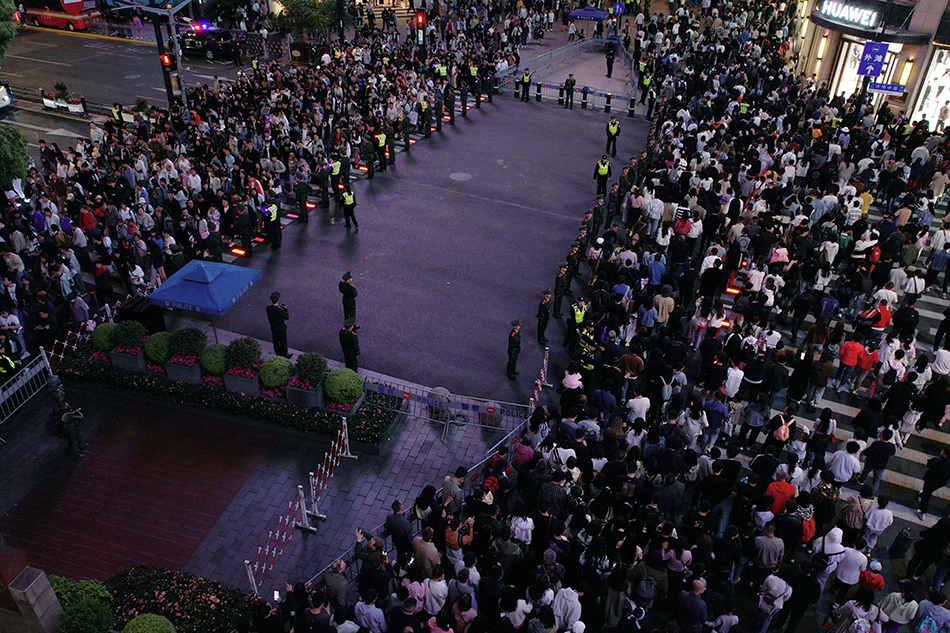
\includegraphics[width=0.47\textwidth]{figures/bund_holiday_crowd.jpeg}
\label{fig:bund_scene_crowd}}
\hfill
\subfloat[]{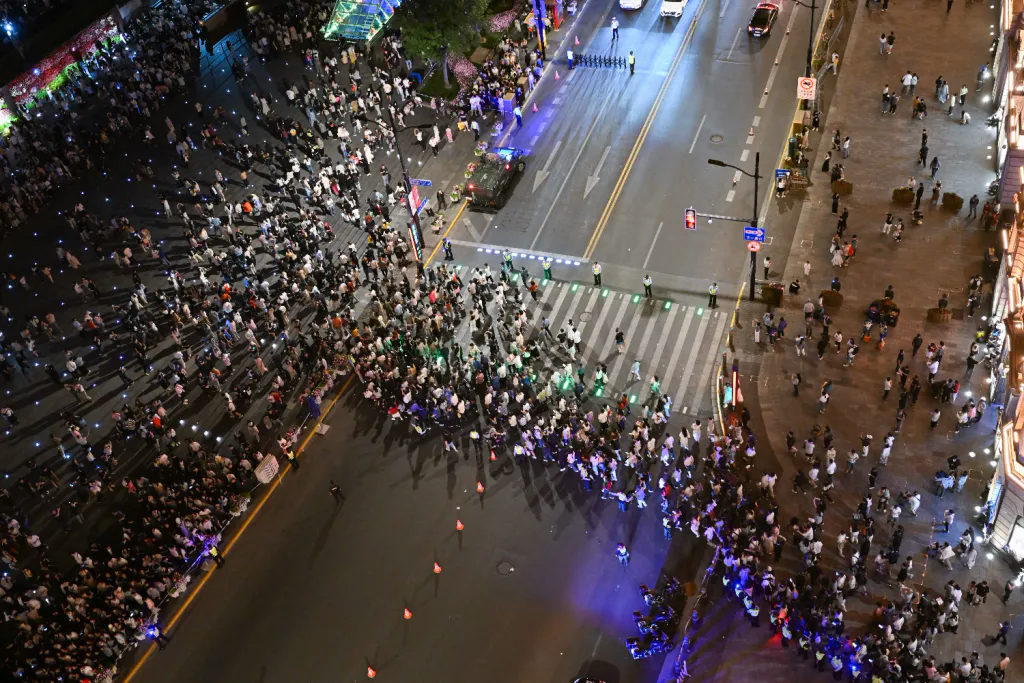
\includegraphics[width=0.47\textwidth]{figures/bund_entrance_control.png}
\label{fig:bund_scene_capacity}}
\figcaptiontight
\caption{Field-control context of the Shanghai Nanjing East Road--Bund area. (a) Large-scale holiday crowd under one-way passage pedestrian flow control on Nanjing East Road; image source: \cite{qq2024huangpu_security}. (b) Entrance-capacity pedestrian flow control link of Bund Passge No.5- Chenyi Square-Nanjing East Road; image source: \cite{chinanews2019bund_flow_guidance}.}
\label{fig:bund_scene}
\end{figure*}

Existing security practice for large events usually combines system-dynamics reasoning, system coupling analysis, high-risk-zone identification, and historical crowd-behavior patterns to design operational controls \cite{RN2176,RN1663}. Typical measures include deploying police or staff at key locations, installing temporary barriers for separation and diversion, enforcing one-way passage rules, and releasing pedestrians in batches into core areas \cite{RN2181,RN1978}. During major holidays, for example, the Shanghai Bund area uses batch release, passage-direction regulation, south-entry--north-exit routing, and conflict-reduction measures \cite{RN2129}. Beijing Nanluoguxiang similarly applies one-way operation on the main street during peak periods, with tourists entering from the south and leaving from the north \cite{RN2130}. These cases share the same control logic: modify local direction and inflow conditions to reorganize pedestrian loads at the area scale.

Despite these practices, high-pedestrian-flow management still depends heavily on manual experience and static contingency plans \cite{RN1662}. Many schemes do not quantitatively describe how passage-direction configurations, entrance release rates, and stage-dependent route preferences shape density evolution. Monitoring based on single-point counts or local density is also insufficient for the coupled process linking passage direction rules, entrance metering, local optimal directions, collective density evolution, and exit-load distribution \cite{RN2124}. In multi-entrance, multi-passage, and multi-stage scenic areas, neglecting route preference and behavioral phase transitions can misjudge passage load and high-risk locations. Moreover, many simulation-optimization studies treat the crowd simulator as an opaque evaluator, rather than exploiting structural information from passage geometry, one-way rules, internal entrance capacities, and multi-route subpopulations \cite{RN2146,RN2122}. This limits search efficiency and makes it difficult to separate whether a candidate strategy works because the underlying control mechanism behaves correctly or because a fixed aggregate score happens to improve.

Therefore, this paper proposes a macroscopic crowd modeling and control optimization framework for the ``Bund sightseeing platform--multi-stepped passage'' open scenic area scenario.
The framework connects multi-stage pedestrian movement, passage direction management, geometric guidance, and entrance release control in one simulation-and-optimization workflow.
It compares candidate strategies under limited simulation budgets, rather than relying only on empirical rules or post-event assessment.

Our main contributions are fourfold:
\begin{enumerate}
\item We formulate a multi-stage, multi-route macroscopic model for the class of open metropolitan tourism hotspots represented by the Bund sightseeing platform and its connected passages. Unlike single-origin--destination or single-potential Hughes-type formulations, the model allows entry, sightseeing, exit, return movement, and route redistribution to interact through shared congestion.

\item We develop a Bellman--conservation-law operator that unifies passage-direction regulation, anisotropic mobility guidance, and internal entrance-rate metering. The operator represents one-way, two-way, and closed passages, channel pre-alignment, open-but-metered entrances, and upstream waiting within mass-consistent dynamics.

\item We design a hierarchical constrained mixed-variable black-box optimization framework (HCMBO) for the joint optimization of passage directions and time-phased entrance admission rates. By exploiting the coupling between direction and capacity, HCMBO identifies feasible control policies under a limited simulation budget and compares them through unified high-fidelity rechecking.

\item We establish a mechanism-aware evaluation and scalability protocol. It first verifies the intended effects of direction constraints and geometric guidance, and then evaluates policies in terms of efficiency, high-density exposure, load balance, entrance waiting, and control smoothness. Because the computational dimension depends on the grid and simulation horizon rather than the number of pedestrians represented, the same model structure, numerical scheme, and grid support analysis at the 50,000-pedestrian scale. A scale-transfer analysis shows that only the demand parameters and simulation horizon need to be adjusted.
\end{enumerate}

\section{Related Work}
\label{sec:related}

\subsection{Massive Crowd Management and Control}

Crowd management studies in urban centers have mainly used boundary regulation, facility layout, and decision-making models \cite{RN2000,RN2193}.
Zhong et al. \cite{RN279} designed boundary control strategies for urban traffic-flow networks and proved convergence to uncongested states under disturbances through Lyapunov analysis \cite{RN1196}.
Wadoo and Kachroo \cite{RN280} used advection and diffusion control to prevent blocking and shock waves in one-dimensional evacuation.
Qin \cite{RN277} proposed a unit sliding-mode controller based on integral barrier Lyapunov functions for multi-directional disturbance propagation.
Zhu et al. \cite{RN286} combined policy learning and neural networks to adjust inflow rates and free-flow speeds in heterogeneous corridors.

Infrastructure-based regulation has also been studied.
Obstacle placement can change outflow, velocity, and local density in merging areas \cite{RN1662,RN2145}.
Yang et al. \cite{RN2118,RN2120} used Model Predictive Control (MPC) to optimize barrier lengths at subway bottlenecks and later included entrance limiters, gates, and escalator directions.
Carmona and Paricio-Garcia \cite{RN2119} proposed dynamic exit-choice recommendations using multinomial Logit models, but the approach depends on discrete speed instructions (e.g., ``stop,'' ``walk,'' ``run'') transmitted through electronic wristbands \cite{RN2196}, which are hard to deploy in open urban areas.

Other studies use optimization and reinforcement learning.
Liao et al. \cite{RN2121} formulated fence layout as subset selection.
Subsequent work \cite{RN2122} used long short-term memory (LSTM) features and Proximal Policy Optimization (PPO) \cite{RN2189} for real-time entrance-flow regulation.
Differential Evolution (DE) \cite{RN2190} has been used to optimize guardrail layout and flow guidance in scenarios such as Chengdu East Railway Station, with average travel time and crowd pressure as objectives \cite{RN2123}.

\subsection{Macroscopic Crowd Modeling and Current Discrepancy Analysis}

Macroscopic crowd models treat pedestrian flows as continuous media, offering computational efficiency and analytical tractability compared to microscopic approaches.
Henderson \cite{RN282} first applied fluid dynamics to pedestrian traffic in the early 1970s, comparing crowd motion to the behavior of gas or fluid particles.

Hughes \cite{hughes2003} pioneered a first-order continuum theory for pedestrian flow, in which walking speed depends on local density through a fundamental diagram, and movement direction follows the steepest-descent path of a potential function representing the remaining travel time to exits.
The model links congestion and route choice through this potential.
Ling et al. \cite{RN2078} generalized the Hughes formulation and solved it with a weighted essentially non-oscillatory (WENO) scheme for the conservation law and a fast-sweeping method for the eikonal equation.

Several extensions modify the density, perception, and constraint terms in macroscopic models.
Colombo et al. \cite{RN2097} proposed nonlocal flux models that replace pointwise density with a neighborhood-averaged quantity in the velocity function to account for anticipatory behavior.
Later work included anisotropic perception fields and wall or obstacle boundary effects, together with high-resolution schemes and well-posedness results for architectural domains \cite{RN2080}.
Maury et al. \cite{RN2099} introduced a projection model for the hard incompressibility constraint, formulating the actual velocity as a least-squares projection of the desired velocity onto the set of feasible non-overlapping configurations.
The same idea was later recast as a Wasserstein gradient flow with density constraints \cite{RN2081}, using the Jordan--Kinderlehrer--Otto (JKO) scheme \cite{RN2188} to keep density below its upper bound.

To overcome non-physical behaviors such as supersonic information propagation that may arise in first-order models, Aw and Rascle \cite{RN2103} introduced a second-order model based on a generalized momentum conservation law that preserves anisotropy.
The Aw--Rascle (AR) framework was subsequently adapted to pedestrian flows \cite{RN2104}, where the congestion pressure term successfully reproduces characteristic phenomena including stop-and-go waves and spontaneous lane formation.

Beyond the classical Hughes-type framework, extensions have incorporated control and guidance mechanisms relevant to crowd management.
Anisotropic formulations using mobility tensors have been developed to represent channel geometries and directional preferences \cite{cristiani2016,priuli2015control}, allowing for continuous geometric guidance without explicit prohibition.
Constrained Hamilton-Jacobi-Bellman (HJB) formulations have been employed to model strict directional constraints such as one-way corridors, with the Bellman optimality principle providing a natural framework for unifying anisotropic geometric guidance with discrete directional constraints.

Despite these advances, three gaps remain for large open scenic areas.
First, Hughes-type single-potential models are destination-oriented and describe one population evacuating toward fixed exits \cite{hughes2003,RN2078}; they cannot represent the multi-stage chain of entering, touring, leaving, and returning, in which subpopulations with stage-dependent goals share the same congested space.
Second, most macroscopic extensions refine the description of flow \cite{RN2097,RN2099,RN2104}, whereas the operational levers used in practice, switching passages among one-way, two-way, and closed states and metering entrance release, are treated as fixed boundary conditions rather than as a joint discrete--continuous decision space \cite{RN2118,RN2122}.
Third, local density or single-point counts are insufficient for such coupled systems \cite{RN2124}; strategy assessment requires area-level indicators linking regional density, passage loads, entrance queues, and exit allocation, which few macroscopic studies provide.
These gaps motivate the multi-stage operator, the joint direction--capacity control space, and the evaluation protocol of this paper.

\section{Methodology}
\label{sec:model}

\subsection{Problem Definition and Overall Framework}

We address a multi-channel crowd management problem in open scenic areas.
The proposed method combines a Bellman--conservation-law crowd dynamics model \cite{hughes2003,RN2078} with a joint direction-capacity control formulation.
The controllable management variable is defined as
\begin{equation}
z=(s,q)\in\mathcal Z,
\label{eq:control_variable}
\end{equation}
where $s$ denotes the discrete direction states of the channels, and $q$ denotes the time-varying internal entrance capacity profile.
The behavioral preference parameter $\hat p$ and the geometric guidance parameter $\eta_0$ are treated as fixed model inputs.
For a given control variable $z$, the lower-level simulator returns density fields, velocity fields, entrance waiting, and realized channel throughputs.
The upper-level optimizer then evaluates efficiency, safety, load balance, waiting, and smoothness metrics, and searches for a better control policy under a limited simulation budget.
The overall method framework is shown in Fig.~\ref{fig:method_framework}.

\begin{figure*}[!t]
\centering
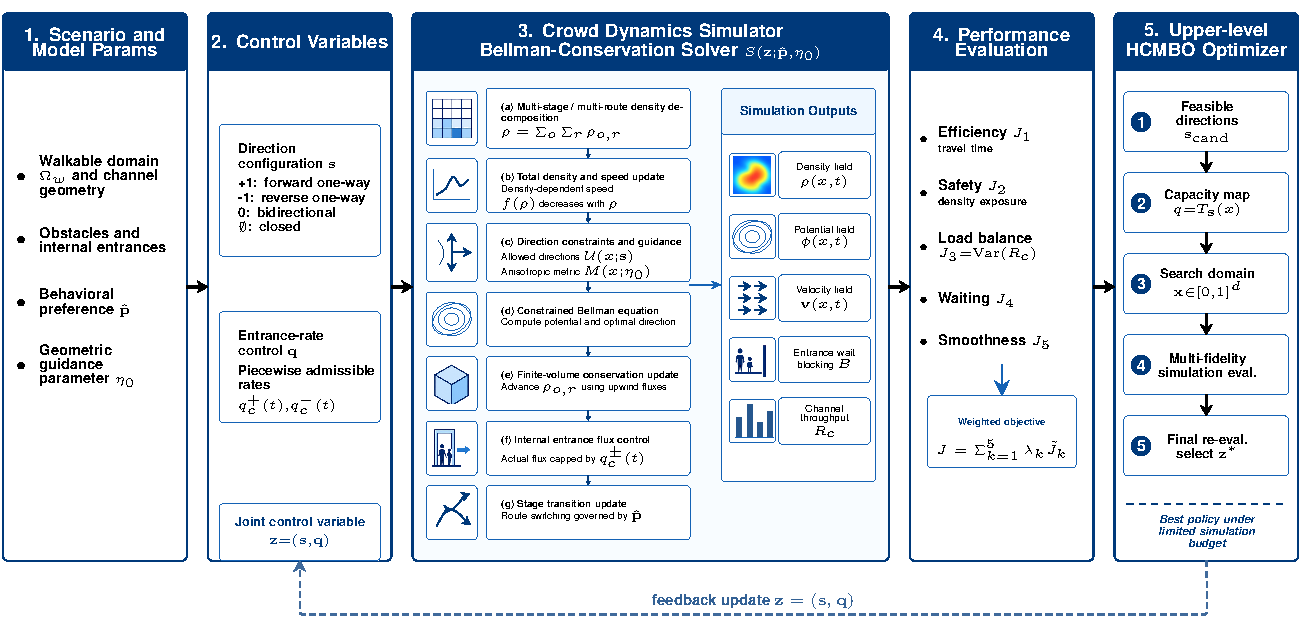
\includegraphics[width=\textwidth]{figures/method_framework.pdf}
\figcaptiontight
\caption{Method framework for joint direction and entrance-rate optimization. Fixed scenario inputs, behavioral preferences, and geometric guidance parameters define the lower-level Bellman--conservation-law crowd simulator. The controllable direction configuration and entrance-rate profile are jointly evaluated by efficiency, safety, load-balance, waiting, and smoothness objectives, and are updated by the upper-level HCMBO optimizer.}
\label{fig:method_framework}
\end{figure*}

We model direction rules and entrance capacities as coupled controls.
The direction configuration $s$ changes the local feasible direction set, whereas the entrance capacity $q$ changes the realized admitted flux at channel entrances.
Together, they affect channel loading, high-density exposure, and upstream waiting.
We therefore formulate crowd management as a mixed-variable simulation-based optimization problem, rather than solving direction selection and capacity assignment as two independent subproblems \cite{RN2122,jiang2018coordinated_inflow,liu2021queuing_network_flow_control}.

\subsection{Bellman--Conservation-Law Crowd Dynamics}

\subsubsection{Conservation Law and Speed Function}

We consider a bounded two-dimensional domain $\Omega \subset \mathbb{R}^2$ representing the pedestrian walking area.
Let $\Omega_w\subset\Omega$ denote the walkable region, $\rho(x,t)$ the total crowd density, and $\mathbf v(x,t)$ the local mean velocity.
Mass conservation is governed by
\begin{equation}
\frac{\partial \rho}{\partial t} + \nabla \cdot (\rho \mathbf{v}) = 0.
\label{eq:continuity}
\end{equation}

The speed magnitude is determined by local congestion.
We adopt the Greenshields-type speed function
\begin{equation}
f(\rho) = v_{\max}\left(1 - \frac{\rho}{\rho_{\max}}\right)_+,
\label{eq:greenshields}
\end{equation}
where $v_{\max}$ is the free-flow speed, $\rho_{\max}$ is the maximum admissible density, and $(\cdot)_+$ denotes nonnegative truncation.
This function captures the feedback that pedestrians move close to free-flow speed in low-density regions and slow down as density approaches congestion.

The classical Hughes model assumes that all movement directions are feasible and isotropic \cite{hughes2003}.
This assumption is insufficient for crowd management scenarios involving one-way rules, temporary closures, entrance metering, and channel-axis alignment.
The following subsections introduce admissible direction sets, anisotropic mobility tensors, and internal entrance capacity control into the Bellman--conservation-law framework.

\subsubsection{Multi-Stage Multi-Route Density Decomposition}

Visitors in open scenic areas usually experience several behavioral stages, such as entry, touring, exit, and return.
To represent this behavior chain, the total density is decomposed into stage--route subpopulations:
\begin{equation}
\rho(x,t) = \sum_{\sigma=1}^{S} \sum_{r=1}^{R_\sigma} \rho_{\sigma,r}(x,t),
\label{eq:density_decomp}
\end{equation}
where $\sigma$ denotes the behavioral stage and $r$ denotes the route type within that stage.
All subpopulations share the speed function $f(\rho)$ determined by the total density, but they have different target regions, potential functions, and velocity directions.

For subpopulation $(\sigma,r)$, the density evolves according to
\begin{equation}
\frac{\partial \rho_{\sigma,r}}{\partial t}
+ \nabla \cdot (\rho_{\sigma,r}\mathbf v_{\sigma,r})
= Q^{\mathrm{in}}_{\sigma,r}-Q^{\mathrm{out}}_{\sigma,r}.
\label{eq:subpop_continuity}
\end{equation}
If pedestrians in subpopulation $(\sigma,r)$ complete the current stage in target region $G_{\sigma,r}$ and switch to next-stage route $k$ with probability $\hat p_{(\sigma,r)\to k}$, the transition term is
\begin{equation}
Q_{(\sigma,r)\to(\sigma+1,k)}(x,t)
=
\hat p_{(\sigma,r)\to k}
\kappa_{\sigma,r}
\chi_{G_{\sigma,r}}(x)
\rho_{\sigma,r}(x,t),
\label{eq:transition}
\end{equation}
where $\kappa_{\sigma,r}$ is the stage-switching rate, with dimension of inverse time, and $\chi_{G_{\sigma,r}}$ is the indicator function of the completion region.
The parameter $\hat p$ represents historically inferred or scenario-given route preferences and is fixed in the optimization problem \cite{RN2302,RN2301,RN2303}.

\subsection{Direction Constraints and Geometric Guidance}

\subsubsection{Direction Configuration Variable}
\label{sec:hjb}

Let the direction state of channel $c$ be
\begin{equation}
s_c \in \{+1,-1,0,\varnothing\},
\label{eq:channel_state}
\end{equation}
where $+1$, $-1$, $0$, and $\varnothing$ denote reference forward one-way, reference reverse one-way, bidirectional, and closed states, respectively.
If $\tau_c(x)$ is the reference tangent direction of channel $c$, the local admissible direction set in the channel region is defined as
\begin{equation}
U_c(x;s_c)=
\begin{cases}
\{\tau_c(x)\}, & s_c=+1,\\
\{-\tau_c(x)\}, & s_c=-1,\\
\{\tau_c(x),-\tau_c(x)\}, & s_c=0,\\
\varnothing, & s_c=\varnothing,
\end{cases}
\quad x\in\Omega_c .
\label{eq:channel_admissible_set}
\end{equation}
Thus, $s_c$ changes the local feasible direction set.
A closed channel has no admissible direction, a one-way channel retains only one reference tangent, and a bidirectional channel retains both opposite tangential directions.

\subsubsection{Anisotropic Mobility Tensor}
\label{sec:guidance}

The admissible set $U(x;s)$ represents hard feasibility, but it does not capture the soft geometric guidance induced by narrow channels.
Pedestrians approaching a channel often pre-align with the channel axis before entering it.
To represent this effect, an anisotropic mobility tensor $M(x;\eta_0)$ is introduced \cite{RN2080,cristiani2016,priuli2015control}.
Equivalently, it is the inverse of a local travel-cost metric.
For channel $c$, let $\tau_c$ and $n_c$ denote its tangent and normal directions.
The mobility tensor is defined as
\begin{equation}
M_c(x;\eta_0)=\beta_c\left(\eta_0\,\tau_c\tau_c^\top+n_c n_c^\top\right),
\qquad \eta_0\ge 1,
\label{eq:mobility_tensor}
\end{equation}
where $\beta_c$ is a channel weight and $\eta_0$ controls the mobility preference strength along the channel axis.
Larger $\eta_0$ increases tangential mobility, equivalently reducing the effective cost of tangential motion and promoting upstream pre-alignment.
The parameter $\eta_0$ is fixed and is not optimized as a control variable.

\subsubsection{Constrained Bellman Equation}

Given $U(x;s)$ and $M(x;\eta_0)$, the potential function $\phi(x,t)$ represents the minimum remaining cost to the corresponding target region.
The discrete Bellman update is
\begin{equation}
\phi(x)=
\min_{\mathbf u\in U(x;s)}
\left[
\phi(x+\Delta x\,\mathbf u)
+\frac{\Delta x}{f(\rho(x,t))}
\frac{1}{\sqrt{\mathbf u^\top M(x;\eta_0)\mathbf u}}
\right].
\label{eq:bellman}
\end{equation}
The optimal direction is
\begin{equation}
\mathbf u^*(x,t)=\operatorname*{arg\,min}_{\mathbf u\in U(x;s)}(\cdots),
\label{eq:optimal_direction}
\end{equation}
and the velocity is
\begin{equation}
\mathbf v(x,t)=f(\rho(x,t))\,\mathbf u^*(x,t).
\label{eq:velocity}
\end{equation}
For the multi-stage multi-route model, each subpopulation $(\sigma,r)$ uses its own target-specific potential $\phi_{\sigma,r}$ while sharing the same total-density congestion feedback.
Thus, direction rules, geometric guidance, and density-dependent congestion are coupled in a single Bellman--conservation-law model.

\subsection{Internal Entrance Capacity Control}

Direction rules alone cannot represent the management action in which a channel is open but its entrance must be metered \cite{jiang2018coordinated_inflow,liu2021queuing_network_flow_control,hu2025passenger_capacity_allocation}.
For each channel, we introduce maximum internal entrance rates
\begin{equation}
q=\{q_c^+(t),q_c^-(t)\}_{c=1}^C,
\label{eq:q_control}
\end{equation}
where $q_c^+(t)$ and $q_c^-(t)$ denote the maximum admitted rates at the reference forward and reverse entrances of channel $c$.
These controls act on internal channel entrance fluxes rather than on external boundary inflows.
In physical units, both the attempted flux $A_c^\pm(t)$ and the capacity bound $q_c^\pm(t)$ are entrance flow rates measured in ped/s.

The direction state and entrance capacity must satisfy the hard consistency constraints
\begin{equation}
\begin{aligned}
s_c=+1 &\Rightarrow q_c^-(t)=0,\\
s_c=-1 &\Rightarrow q_c^+(t)=0,\\
s_c=\varnothing &\Rightarrow q_c^+(t)=q_c^-(t)=0,\\
s_c=0 &\Rightarrow q_c^+(t)+q_c^-(t)\le \bar q_c.
\end{aligned}
\label{eq:direction_capacity_consistency}
\end{equation}
Let $A_c^\pm(t)$ be the attempted entrance flux induced by free movement.
The actually admitted flux is
\begin{equation}
\hat A_c^\pm(t)=\min\{A_c^\pm(t),q_c^\pm(t)\}.
\label{eq:admitted_flux}
\end{equation}
When $A_c^\pm(t)>0$, the flux across the internal entrance is scaled by
\begin{equation}
\theta_c^\pm(t)=\frac{\hat A_c^\pm(t)}{A_c^\pm(t)}.
\label{eq:flux_scaling}
\end{equation}
The excess demand $(A_c^\pm(t)-\hat A_c^\pm(t))_+$ remains upstream and is recorded as waiting or queueing mass.
This treatment changes channel usage and risk distribution while preserving the mass balance of the conservation-law update.

\subsection{Numerical Solver and Simulation Operator}
\label{sec:numerical}

The walkable region, obstacles, channel areas, and internal entrance interfaces are discretized on a uniform two-dimensional grid.
At each time step, the total density is first computed from all stage--route subpopulations and used to update $f(\rho)$.
For each subpopulation, the admissible direction set and mobility tensor are then constructed, and the corresponding discrete Bellman equation is solved.
After the velocity direction is recovered, an upwind finite-volume update advances the conservation law, while internal entrance fluxes are modified by $\theta_c^\pm(t)$ \cite{RN2078}.
Finally, stage transition terms are applied to update the subpopulation densities.

For any feasible control variable $z=(s,q)$, the complete numerical workflow defines a lower-level simulation operator
\begin{equation}
(\rho,\phi,\mathbf v,B,R)=\mathcal S(z;\hat p,\eta_0),
\label{eq:simulation_oracle}
\end{equation}
where $B$ records entrance waiting or blocking and $R=(R_1,\ldots,R_C)$ records realized cumulative throughputs of the channels.
The channel balance metric below is computed from the realized throughputs $R_c$, not from the prescribed capacity limits $q_c^\pm(t)$.

\subsection{Evaluation Metrics and Optimization Objective}
\label{sec:metrics}

\subsubsection{Efficiency, Safety, and Load Balance}

Following recent passenger-flow-control and crowd-evacuation simulation-optimization studies \cite{RN2145,RN2119,hu2025passenger_capacity_allocation}, the total travel time metric is
\begin{equation}
J_1(z) = \int_0^T \int_{\Omega_w} \rho(x,t) \, dx \, dt.
\label{eq:j1}
\end{equation}
The high-density exposure metric is
\begin{equation}
J_2(z) = \int_0^T \int_{\Omega_w} \mathbf{1}_{\rho(x,t) > \rho_{\text{safe}}} \, dx \, dt.
\label{eq:j2}
\end{equation}
The safety threshold is the density above which exposure is counted, and is fixed at $\rho_{\text{safe}}=3.5$~ped/m$^2$ in both the four-channel and Bund scenarios.
Let
\begin{equation}
R_c(T)=\int_0^T(\hat A_c^+(t)+\hat A_c^-(t))\,dt
\label{eq:channel_throughput}
\end{equation}
be the realized cumulative throughput of channel $c$.
The channel load imbalance is
\begin{equation}
J_3(z) = \operatorname{Var}(R_1(T), \dots, R_C(T)).
\label{eq:j3}
\end{equation}

\subsubsection{Entrance Waiting and Control Smoothness}

Entrance waiting is penalized as
\begin{equation}
J_4(z)=\int_0^T\sum_{c=1}^{C}\left(B_c^+(t)+B_c^-(t)\right)\,dt.
\label{eq:j4}
\end{equation}
For piecewise-constant capacity profiles, smoothness is measured by
\begin{equation}
J_5(z)=\sum_{c,k}\left[(q_{c,k+1}^+-q_{c,k}^+)^2+(q_{c,k+1}^--q_{c,k}^-)^2\right].
\label{eq:j5}
\end{equation}
Here $k$ indexes the capacity-control time segment.
$J_4$ discourages excessive entrance metering that creates upstream queues, while $J_5$ discourages abrupt high-frequency changes in capacity profiles \cite{RN2196,jiang2018coordinated_inflow,liu2021queuing_network_flow_control,hu2025passenger_capacity_allocation}.

\subsubsection{Normalization and Scalar Objectives}

The raw metrics above have different physical units and numerical scales.
Therefore, the reported scalar objectives are computed from dimensionless normalized quantities.
Let
\[
M_{\mathrm{ref}}=M_0+M_{\mathrm{in}},\qquad T_e=T,
\]
where $M_0$ is the initial crowd mass, $M_{\mathrm{in}}$ is the cumulative external inflow during $[0,T]$, and $T_e$ is the evaluation horizon.
Let $|\Omega_w|$ be the walkable area, $R_{\mathrm{tot}}=\sum_{c=1}^{C}R_c(T)$, and
\[
D_R=R_{\mathrm{tot}}^2\frac{C-1}{C^2}.
\]
The basic normalized terms are
\[
\bar J_1=\frac{J_1}{M_{\mathrm{ref}}T_e},\qquad
\bar J_2=\frac{J_2}{|\Omega_w|T_e},
\]
\[
\bar J_3=\frac{J_3}{D_R+\varepsilon_R},\qquad
\bar J_4=\frac{J_4}{M_{\mathrm{ref}}T_e}.
\]
For segmented entrance-rate profiles, the smoothness term is normalized by the corresponding entrance-rate bounds:
\[
\bar J_5=
\frac{1}{N_q}
\sum_{c,k,\sigma\in\{+,-\}}
\left(
\frac{q_{c,k+1}^{\sigma}-q_{c,k}^{\sigma}}
{\bar q_c^{\sigma}+\varepsilon_q}
\right)^2 .
\]
Here $N_q$ is the number of active finite differences, $\bar q_c^\sigma$ is the reference upper bound of the corresponding entrance, and $\varepsilon_R$ and $\varepsilon_q$ only avoid zero denominators.
Thus, $\bar J_1$ is a relative system-residence measure.
The term $\bar J_2$ is the average hard exposure or soft safety-risk intensity over the walkable space-time domain \cite{RN2059}.
The term $\bar J_3$ is zero for perfectly balanced realized channel use and approaches one when all realized channel throughput concentrates on one channel.

The reported terms use scale factors
\begin{equation}
\tilde J_k=\frac{\bar J_k}{a_k}.
\label{eq:scaled_terms}
\end{equation}
The main experiments use
\[
(a_1,a_2,a_3,a_4,a_5)=(1,10^{-3},1,1,1).
\]
Therefore, the reported $\tilde J_2$ values are scaled normalized safety terms and should not be read directly as space-time percentages; the basic normalized value is $\bar J_2=10^{-3}\tilde J_2$.
Given weights $\lambda=(\lambda_1,\ldots,\lambda_5)$, the scalarized objective is
\begin{equation}
J(z) = \sum_{k=1}^{5}\lambda_k\tilde{J}_k(z),
\label{eq:scalarized}
\end{equation}
with the main-experiment setting
\[
(\lambda_1,\lambda_2,\lambda_3,\lambda_4,\lambda_5)=(1,1,1,1,0.1).
\]
and the optimization problem is
\begin{equation}
\min_{z \in \mathcal{Z}} J(z), \qquad z=(s,q).
\label{eq:optimization}
\end{equation}
The paper solves this fixed-weight scalarized management problem.
Different weights can represent different management preferences, but the algorithm itself does not depend on one specific objective term being independently optimal.
Although $J$, $J^{(3)}$, and $\tilde J_k$ are dimensionless ranking quantities, their interpretation is anchored by the normalization above \cite{RN2123,marler2004survey_moo_engineering}.
When physical interpretation is needed, the experiments also report raw or ratio-based diagnostics such as channel-flow shares, system mass, and density peaks.
Table~\ref{tab:objective_units} lists the physical units of the raw objective terms and their normalizers; in each case the term and its normalizer share the same unit, so every reported $\tilde J_k$ is dimensionless.

\begin{table}[!t]
\centering
\caption{Raw Units of the Objective Terms and Their Normalizers}
\label{tab:objective_units}
\footnotesize
\setlength{\tabcolsep}{5pt}
\begin{tabular}{l l l l}
\hline
Term & Raw unit & Normalizer (same unit) & Reported \\
\hline
$J_1$ & ped$\cdot$s & $M_{\mathrm{ref}}T_e$ (ped$\cdot$s) & dimensionless \\
$J_2$ & m$^2\cdot$s & $|\Omega_w|T_e$ (m$^2\cdot$s) & dimensionless \\
$J_3$ & ped$^2$ & $D_R$ (ped$^2$) & dimensionless \\
$J_4$ & ped$\cdot$s & $M_{\mathrm{ref}}T_e$ (ped$\cdot$s) & dimensionless \\
$J_5$ & (ped/s)$^2$ & $(\bar q_c^\sigma)^2$ (ped/s)$^2$ & dimensionless \\
\hline
\end{tabular}
\end{table}

For mechanism-verification experiments and fixed-strategy diagnostic experiments that only test direction rules, geometric guidance, or fixed entrance-rate responses, we use the reduced three-term objective
\begin{equation}
J^{(3)}(z)=
\lambda_1\tilde J_1(z)
+\lambda_2\tilde J_2(z)
+\lambda_3\tilde J_3(z).
\label{eq:reduced_objective}
\end{equation}
In these experiments, the entrance-waiting term $\tilde J_4$ is either reported only as a diagnostic quantity or is not applicable, and the smoothness term $\tilde J_5$ is meaningful only for segmented capacity-profile optimization.
Equivalently, reduced-objective experiments use $\lambda_4=\lambda_5=0$.
The numerical values of $J$ and $J^{(3)}$ are not compared across experiment groups.

\subsection{Hierarchical Constrained Mixed-Variable Black-Box Optimization}
\label{sec:optimization}

Since $s$ is discrete, $q$ is continuous or piecewise continuous, and each objective evaluation requires the expensive simulator $\mathcal S$, the resulting problem is an expensive mixed-variable black-box optimization problem \cite{sheikh2022mixed_variable_mobo,ramirez2022mixed_variables_bo,dreczkowski2023mixed_variable_bo}.
We propose HCMBO, a Hierarchical Constrained Mixed-variable Black-box Optimization method, to exploit the structural relation between direction variables and capacity variables.

\subsubsection{Direction Candidates and Capacity Parameterization}

HCMBO first generates a direction candidate set $\mathcal S_{\mathrm{cand}}$ satisfying operational and connectivity constraints.
For a fixed direction configuration $s$, the entrance capacity profile is represented by a low-dimensional continuous vector $x\in[0,1]^d$ and mapped to the actual capacity control by
\begin{equation}
q=T_s(x),\qquad x\in[0,1]^d.
\label{eq:capacity_parameterization}
\end{equation}
The mapping $T_s$ automatically applies direction masks, capacity upper bounds, closure constraints, and smoothness restrictions.
For example, if a channel is set to reference forward one-way, the reverse entrance capacity is set to zero; if a channel is closed, both directional capacities are set to zero.
Thus, the optimizer searches in the continuous $x$-space while all candidates are mapped to capacity profiles consistent with the discrete direction configuration.

\subsubsection{Structured Capacity Search}

For each direction candidate $s$, HCMBO performs structured search in the corresponding capacity parameter space.
The search uses previously evaluated samples to construct surrogate information for objective values and feasibility, and preferentially selects capacity candidates that satisfy constraints and may improve the incumbent objective.
This hierarchical design avoids blind sampling in the full mixed-variable space and separates discrete direction structure from continuous capacity structure.

Multi-fidelity evaluation can be used during search.
Low- or medium-fidelity simulations help identify clearly poor capacity profiles, whereas high-fidelity simulations are reserved for final candidate rechecking and ranking.
To avoid discarding good long-horizon strategies due to short-horizon bias, low-fidelity results are used only as auxiliary evaluation signals and do not directly determine the final optimum.

\subsubsection{High-Fidelity Rechecking and Final Selection}

All finalist candidates are re-evaluated under a unified high-fidelity (HF) setting.
Let $\mathcal C_{\mathrm{HF}}$ be the candidate set selected for high-fidelity rechecking.
The final output is
\begin{equation}
z^*=\operatorname*{arg\,min}_{z\in\mathcal C_{\mathrm{HF}}}J_{\mathrm{HF}}(z).
\label{eq:hcmbo_final}
\end{equation}
This mechanism prevents surrogate error, low-fidelity bias, or intermediate search ranking from directly becoming the final performance claim.

Algorithm~\ref{alg:hcmbo} gives the reproducible HCMBO procedure used in the experiments.
The loop terminates after the finite optimization budget has been allocated across direction candidates, and the reported optimum is selected only after the high-fidelity rechecking stage.

\begin{algorithm}[!t]
\caption{HCMBO for Joint Direction and Entrance-Rate Control}
\label{alg:hcmbo}
\small
\raggedright
\begin{algorithmic}[1]
\REQUIRE Direction constraints $\Omega_s$; simulator $\mathcal S$; objective $J$; gate-rate bounds $\bar q$; budget $B$; initial design size $n_0$; pool size $P$; lower confidence bound (LCB) coefficient $\beta$; high-fidelity shortlist size $K$.
\ENSURE Best high-fidelity policy $z^*$.
\STATE Generate $\mathcal S_{\mathrm{cand}}$ by enumerating $s\in\Omega_s$ and retaining only configurations satisfying open-channel and connectivity constraints.
\STATE Rank $\mathcal S_{\mathrm{cand}}$ using the prescribed priority templates and direction proxy score, and then truncate it to the direction-candidate limit.
\STATE Set $b_s=\lfloor B/|\mathcal S_{\mathrm{cand}}|\rfloor$ and assign one extra evaluation to the first $B\bmod|\mathcal S_{\mathrm{cand}}|$ directions.
\STATE Initialize the global evaluation log $\mathcal D\leftarrow\emptyset$.
\FORALL{$s\in\mathcal S_{\mathrm{cand}}$}
\STATE Construct $T_s:[0,1]^{d_s}\rightarrow q$ by applying the direction mask, gate bounds $\bar q$, and time segmentation.
\STATE Initialize $\mathcal D_s\leftarrow\emptyset$ and generate $X_s^{0}$ from high-, medium-, and low-rate profiles plus random fill-up points.
\FORALL{$x\in X_s^{0}$}
\IF{$|\mathcal D_s|<b_s$}
\STATE Evaluate $z=(s,T_s(x))$ with the optimization-fidelity simulator and append $(x,z,J(z))$ and feasibility metrics to $\mathcal D_s$ and $\mathcal D$.
\ENDIF
\ENDFOR
\WHILE{$|\mathcal D_s|<b_s$}
\STATE Let $x_s^{\mathrm{best}}$ be the evaluated point with the lowest objective in $\mathcal D_s$.
\STATE Draw $\mathcal P_s$ from $P$ uniform samples in $[0,1]^{d_s}$ and $\max(4,\lfloor P/4\rfloor)$ Gaussian perturbations of $x_s^{\mathrm{best}}$, clipped to $[0,1]^{d_s}$.
\STATE Set the kernel length scale $\ell_s=\max\{0.18,1/\sqrt{d_s}\}$.
\FORALL{$u\in\mathcal P_s$}
\STATE Estimate $\hat\mu_s(u)$ by weighted averaging with $w_i(u)=\exp(-\|x_i-u\|_2^2/(2\ell_s^2))$ over $(x_i,z_i,J_i)\in\mathcal D_s$.
\STATE Set $\hat\sigma_s(u)=\min\{1,\min_{(x_i,z_i,J_i)\in\mathcal D_s}\|u-x_i\|_2/\sqrt{d_s}\}$.
\STATE Compute $a_s(u)=\hat\mu_s(u)-\beta\,\operatorname{std}(\mathcal D_s)\hat\sigma_s(u)$.
\ENDFOR
\STATE Select $x_{\mathrm{next}}\leftarrow\arg\min_{u\in\mathcal P_s}a_s(u)$.
\STATE Evaluate $z_{\mathrm{next}}=(s,T_s(x_{\mathrm{next}}))$ and append the result to $\mathcal D_s$ and $\mathcal D$.
\ENDWHILE
\ENDFOR
\STATE Select the top $K$ unique controls $\mathcal C_{\mathrm{HF}}$ from $\mathcal D$ by the optimization-fidelity objective.
\FORALL{$z\in\mathcal C_{\mathrm{HF}}$}
\STATE Re-evaluate $z$ under the unified high-fidelity simulator setting to obtain $J_{\mathrm{HF}}(z)$.
\ENDFOR
\RETURN $z^*=\operatorname*{arg\,min}_{z\in\mathcal C_{\mathrm{HF}}}J_{\mathrm{HF}}(z)$.
\end{algorithmic}
\end{algorithm}

Compared with generic mixed-variable optimization, HCMBO uses the dependence between direction choices and feasible capacity profiles.
Once $s$ is fixed, the mapping $T_s$ removes capacity variables that conflict with the selected direction rules and bounds the remaining entrance-rate profiles.
This reduces invalid candidates and allocates the simulation budget to policies that satisfy the operational constraints.


\section{Numerical Experiments}
\label{sec:experiments}

We validate the proposed model and optimizer on a four-channel scenic-platform scenario abstracted from the Bund sightseeing platform setting.
The scenario consists of an inflow region, a Bund sightseeing platform and exit region, a central wall, and four connecting channels: upper, middle, lower-middle, and bottom channels.
Throughout this paper, channel denotes a model flow entity indexed by $c$, whereas passage refers to a real-world walkway at the Bund site that a channel abstracts.
The experiments are organized as mechanism validation, directional-response analysis, entrance-rate response, horizontal optimizer comparison, and HCMBO ablation.

\subsection{Experimental Setup}
\label{sec:setup}

The domain is discretized on a $128\times96$ grid.
To report results in physical units, simulation quantities are mapped through a representative calibration based on three reference scales: a grid cell size of $\Delta x=1.0$~m, so that the domain spans $128~\mathrm{m}\times96~\mathrm{m}$; a free-flow walking speed of $1.5$~m/s; and a jam density of $5.0$~ped/m$^2$.
The induced time step is then $\Delta t=0.2$~s, and pedestrian counts follow by integrating density over physical area, so that a fully occupied cell holds $\rho_{\max}\Delta x^2=5$~ped. As a coherence check, a fully packed domain of this size would hold at most $\rho_{\max}\times128\times96\approx6.1\times10^4$~ped, which bounds all reported pedestrian counts.
These physical units are adopted only for readability and reflect a representative assumption; they do not represent any specific venue.

The channel width is $4$~m, and the controlled internal entrance interface width is $16$~m.
The free-flow speed is $v_{\max}=1.5$~m/s, the maximum density is $\rho_{\max}=5.0$~ped/m$^2$, the initial density is $\rho_{\mathrm{init}}=2.2$~ped/m$^2$, and the Courant--Friedrichs--Lewy (CFL) factor is $0.9$.

Mechanism and response experiments use the corresponding validation horizons.
The optimizer comparison uses high-fidelity rechecks with $1600$ simulation steps, a horizon of $320$~s (i.e. $\Delta t=0.2$~s), and Bellman updates every five steps.
Final optimizer rankings are based on the high-fidelity objective in Section~\ref{sec:metrics}.
Unless otherwise stated, optimization experiments are ranked by the full five-term scalar objective $J$ after high-fidelity rechecking.

Mechanism-validation, directional-response, fixed-rate response, and supplementary transfer diagnostics use the reduced objective $J^{(3)}=\lambda_1\tilde J_1+\lambda_2\tilde J_2+\lambda_3\tilde J_3$.
For these reduced-objective experiments, $\tilde J_4$ is only an entrance-waiting diagnostic or is not applicable, and $\tilde J_5$ is not applicable.
Equivalently, $\lambda_4=\lambda_5=0$.
Therefore, the numerical values of $J$ and $J^{(3)}$ should not be compared across experiment groups.
Comparisons are meaningful only within the same objective definition, normalization rule, and weight setting.
A high-fidelity best candidate is called feasible if the density-cap removal mass is no more than $2\%$ of the reference mass.

Unless otherwise stated, cumulative flow, waiting mass, unreleased attempted flow, and system mass are reported in pedestrians (ped), obtained by integrating density over the physical cell area.
Mass-time quantities are reported in ped$\cdot$s.
Counterflow area-time is reported in m$^2\cdot$s.
Channel-flow shares are computed from realized cumulative channel throughputs, $R_c(T)/\sum_jR_j(T)$.
Scalar objectives and normalized terms are dimensionless.
Raw cumulative quantities are rounded to three significant digits in the text, while tables retain four decimals for dimensionless objective terms.

\begin{figure}[!t]
\centering
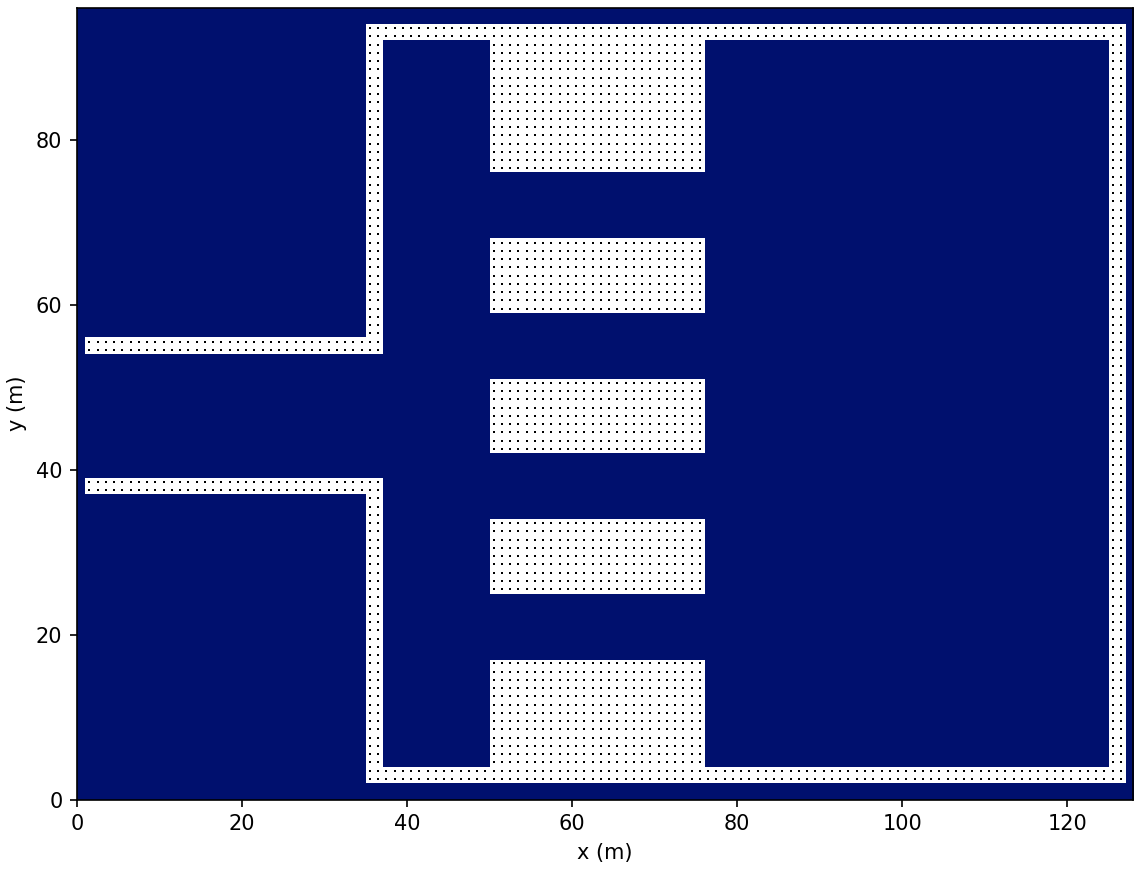
\includegraphics[width=\columnwidth]{figures/scene.png}
\figcaptiontight
\caption{Four-channel scenic-platform simulation scenario used in the numerical experiments.}
\label{fig:experiment_scene}
\end{figure}

\subsection{Mechanism Validation}
\label{sec:mechanism}

We first verify whether the two local modeling components have the intended behavioral meanings.
The fixed anisotropic mobility tensor $M(x;\eta_0)$ should reshape the channel attraction domain and induce entrance pre-alignment, whereas the admissible direction set $U(x;s)$ should remove prohibited directions and reroute flow through feasible channels.
When $M$ is applied to the middle channel, its flow share increases from $48.78\%$ in the baseline to $100.00\%$.
When a one-way rule excludes the originally dominant middle-channel direction, the middle-channel share becomes zero and the flow is redistributed to the upper, lower-middle, and bottom channels with shares $19.25\%$, $68.76\%$, and $12.00\%$, respectively.
For the bidirectional validation case, we use two diagnostic quantities.
The reverse-direction mass time (RMT) is
\[
\mathrm{RMT}=
\sum_n\sum_{i\in\Omega_c}
\rho_i^n
\mathbf 1\{\mathbf u_i^n\cdot\tau_c<0\}
\Delta x^2\Delta t,
\]
which measures the cumulative reverse-direction mass-time (in ped$\cdot$s) moving against the prescribed channel direction.
The counterflow area-time (CAT) is
\[
\mathrm{CAT}=
\sum_n\sum_{i\in\Omega_c}
\mathbf 1\{\rho_{i,+}^n>0,\rho_{i,-}^n>0\}\,\Delta x^2\Delta t,
\]
which measures the cumulative area-time (in m$^2\cdot$s) during which opposite-direction subpopulations coexist in the same channel region.
In the baseline bidirectional inflow test, the westbound middle-channel share, RMT, and CAT are $73.18\%$, $3.33\times10^{3}$~ped$\cdot$s, and $2.43\times10^{3}$~m$^2\cdot$s, respectively.
After imposing the eastbound one-way rule, all three quantities are reduced to zero.

\begin{figure*}[!t]
\centering
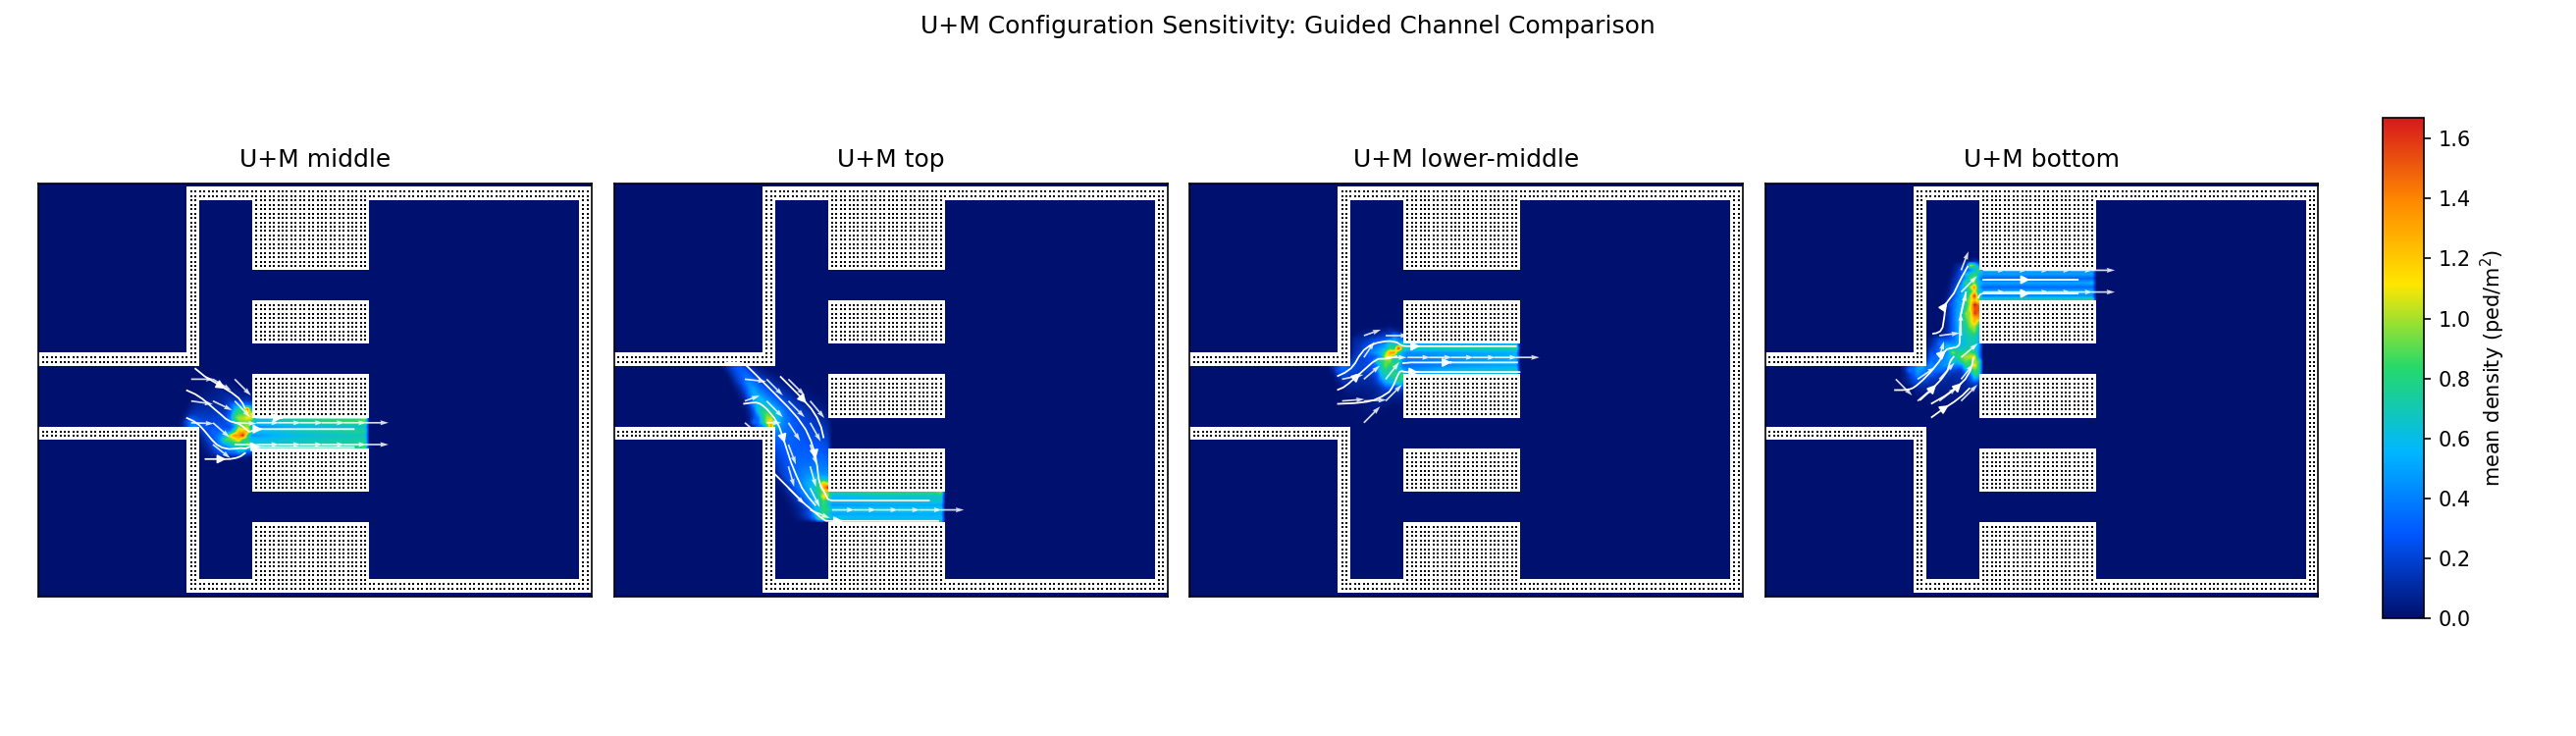
\includegraphics[width=0.82\textwidth]{figures/g1_flow_comparison.png}
\figcaptiontight
\caption{Spatial transferability of the combined $U+M$ mechanism. Moving the controlled channel induces corresponding migration of dominant flow channels, streamlines, and density hotspots.}
\label{fig:g1_um_configuration}
\end{figure*}

Fig.~\ref{fig:g1_um_configuration} compares guidance applied to different channels.
In each case, the dominant flow channel and local density hotspot move with the guided channel.
This supports using the Bellman--conservation-law simulator as the lower-level evaluator for subsequent strategy optimization.

\subsection{Directional-Control Response}
\label{sec:strategy}

We next examine whether the discrete direction configuration $s$ creates nontrivial system-level trade-offs.
The response experiment uses thirteen interpretable direction settings: an all-free baseline, four single-entry cases, four single-return cases, and four one-channel-closure cases.
The direction code is ordered as $[T,M,LM,B]$, representing the top, middle, lower-middle, and bottom channels, where $E$, $W$, $F$, and $X$ denote eastbound entry, westbound return, bidirectional free channel, and closure.
Policy labels use baseline (BSL), single-entry (SE), and single-return (SR), with suffixes identifying the affected channel.

\begin{figure*}[!t]
\centering
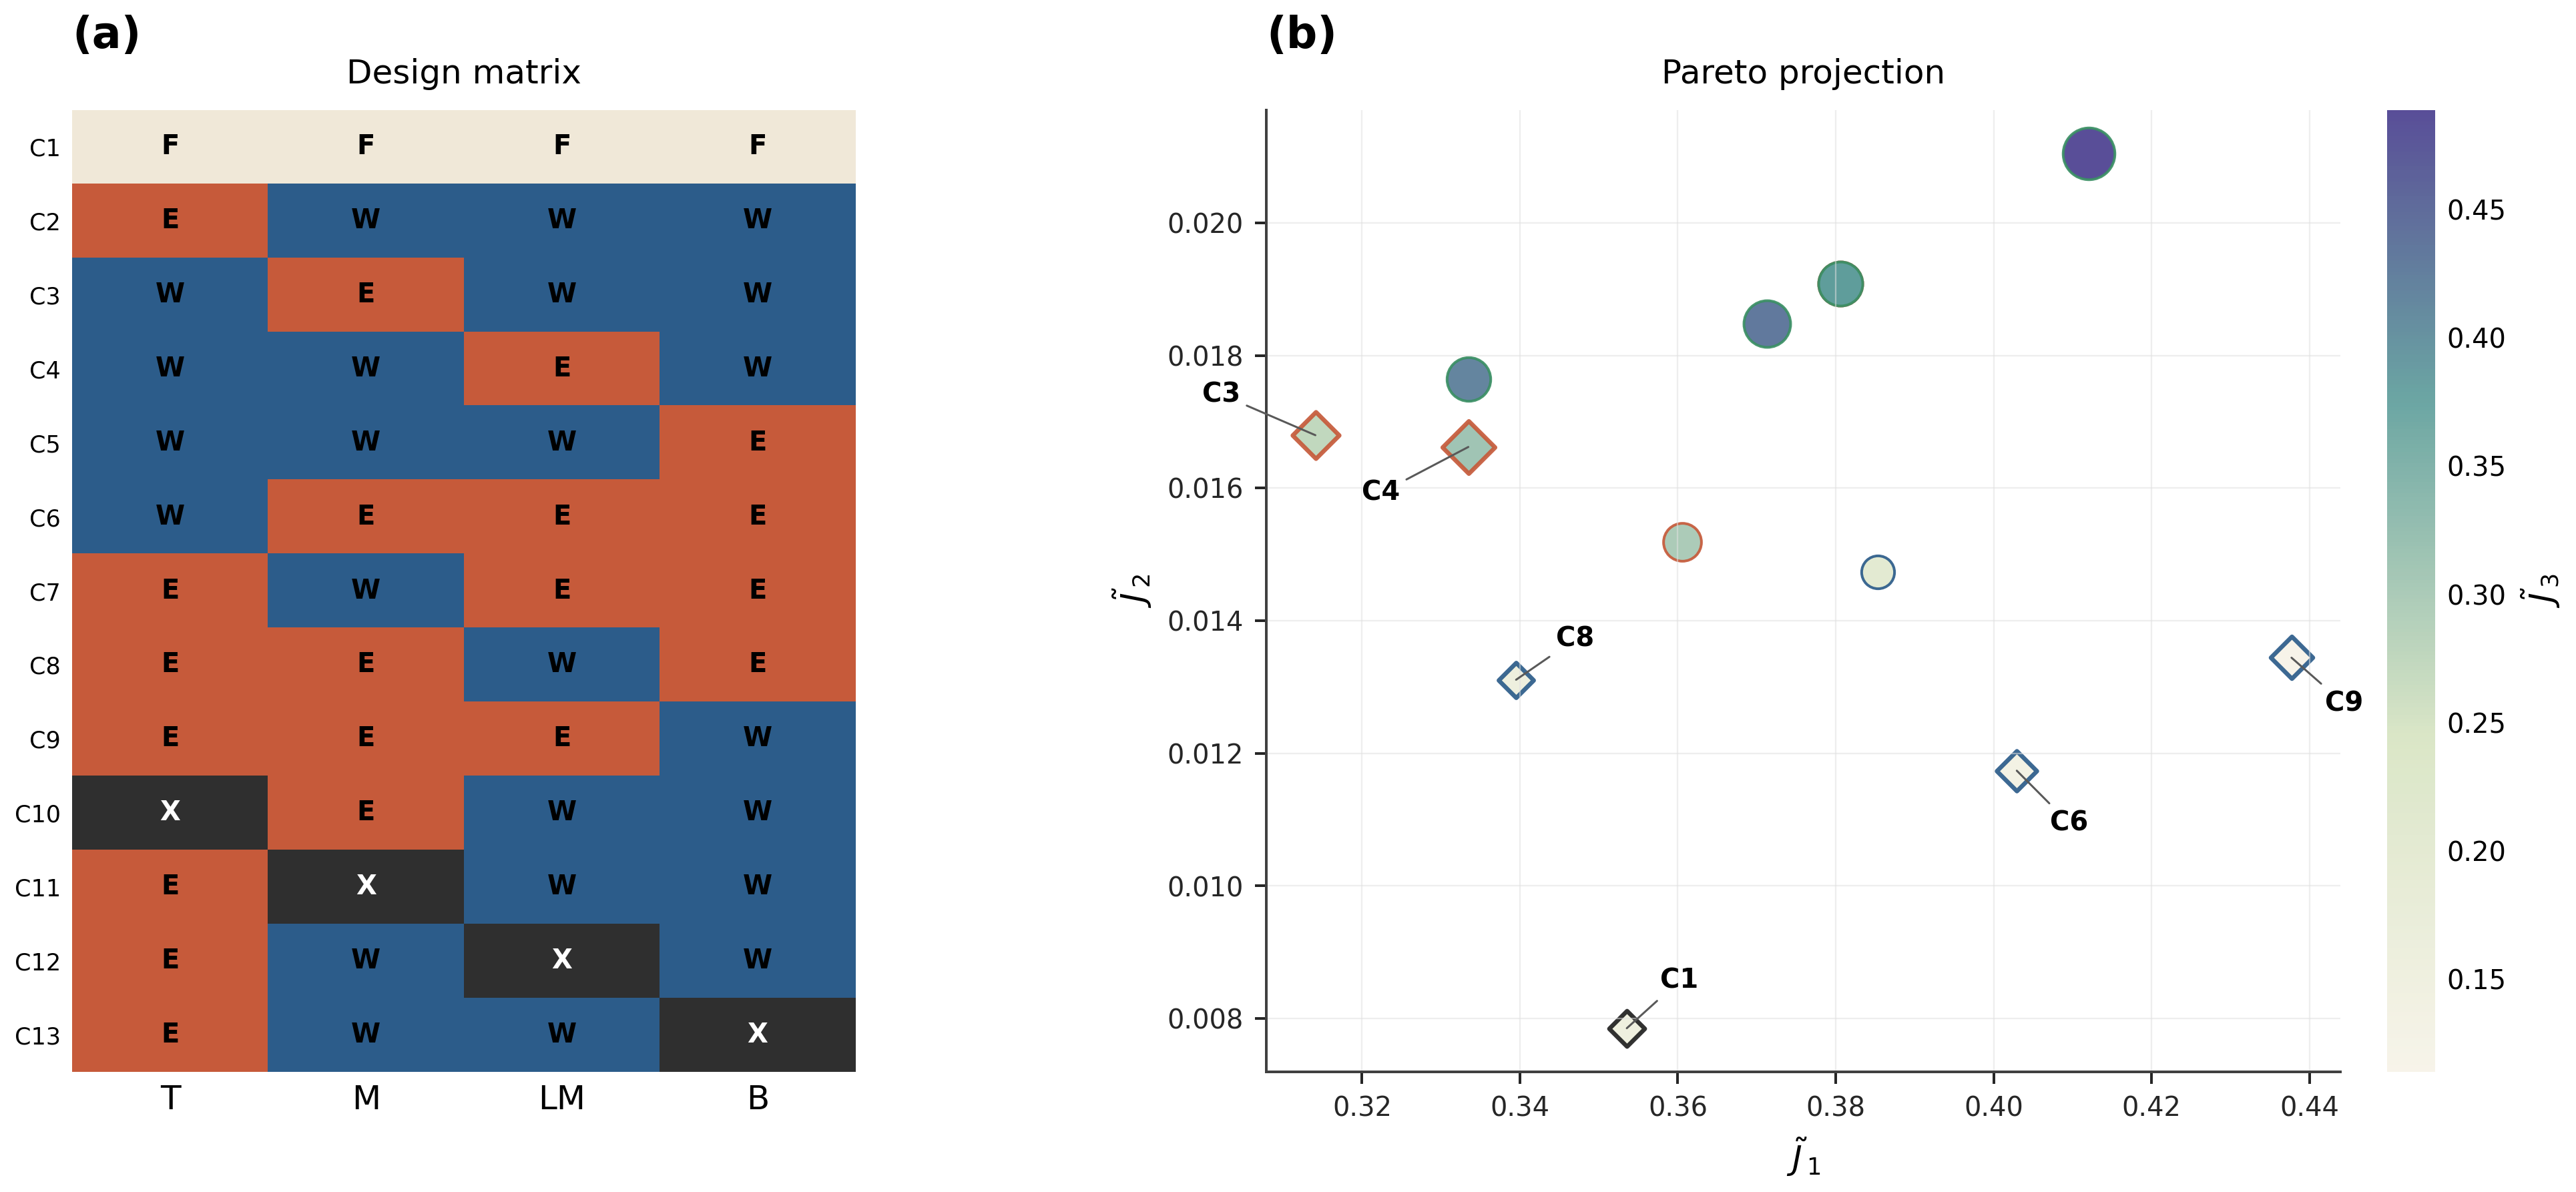
\includegraphics[width=0.92\textwidth]{figures/g2_tradeoff_summary.png}
\figcaptiontight
\caption{Directional-control design matrix and objective-space trade-off. Color encodes $\tilde J_3$, marker size encodes the reduced dimensionless diagnostic objective $J^{(3)}$, and diamonds indicate non-dominated cases.}
\label{fig:g2_control_tradeoff}
\end{figure*}

Fig.~\ref{fig:g2_control_tradeoff} and Table~\ref{tab:g2_nondominated} show that no single direction configuration dominates all objectives.
This directional-response experiment summarizes the three reported terms by $J^{(3)}$; since no entrance-capacity curve is optimized, $\tilde J_4$ and $\tilde J_5$ are not used for ranking.
C8 (SR-LM, EEWE) obtains the lowest reduced objective $J^{(3)}=0.5102$, which is only $0.84\%$ lower than the all-free baseline C1.
C1 gives the lowest safety exposure $\tilde J_2=0.00785$, C3 gives the best efficiency term $\tilde J_1=0.3141$, and C9 gives the best load-balance term $\tilde J_3=0.1138$.
This non-monotonic response makes manual rule selection from a small set insufficient and motivates automatic mixed-variable optimization.

\begin{table}[!t]
\centering
\caption{Non-Dominated Directional-Control Cases}
\label{tab:g2_nondominated}
\footnotesize
\setlength{\tabcolsep}{2pt}
\makebox[\columnwidth][c]{%
\renewcommand{\arraystretch}{1.12}%
\setlength{\extrarowheight}{0.6pt}%
\begin{tabular}{@{}c c c r r r r >{\raggedright\arraybackslash}m{0.22\columnwidth}@{}}
\hline
Case & Policy & Code & $\tilde J_1$ & $\tilde J_2$ & $\tilde J_3$ & $J^{(3)}$ & Main characteristic \\
\hline
C1 & BSL & FFFF & 0.3535 & \textbf{0.00785} & 0.1531 & 0.5145 & Lowest exposure \\
C3 & SE-M & WEWW & \textbf{0.3141} & 0.01680 & 0.2741 & 0.6049 & Best efficiency but risk-concentrated \\
C4 & SE-LM & WWEW & 0.3335 & 0.01662 & 0.3131 & 0.6632 & Efficient but load-imbalanced \\
C6 & SR-T & WEEE & 0.4029 & 0.01174 & 0.1335 & 0.5482 & High return throughput \\
C8 & SR-LM & EEWE & 0.3395 & 0.01311 & 0.1576 & \textbf{0.5102} & Lowest reduced objective \\
C9 & SR-B & EEEW & 0.4377 & 0.01344 & \textbf{0.1138} & 0.5649 & Most balanced channel loads \\
\hline
\end{tabular}
}
\par\vspace{3.5mm}
\noindent\parbox{\columnwidth}{\footnotesize All objective terms in this table are dimensionless scaled normalized quantities. The reduced objective uses $\lambda_4=\lambda_5=0$ and is used only for directional-response diagnosis; it is not directly comparable with the full five-term objective in Table~\ref{tab:optimizer_summary}.}
\end{table}

\subsection{Entrance-Rate Response}
\label{sec:entrance_rate_exp}

Direction rules alone cannot represent the case in which a channel remains open but its internal entrance must be metered.
We therefore fix $[T,M,LM,B]=[F,E,W,F]$ and scan four internal entrance-rate levels: no limit, high, medium, and low.
The rate upper bound acts on internal entrance crossing flow.
When attempted flow exceeds the upper bound, only the admitted flow crosses the interface, and the unreleased attempted flow remains upstream as waiting mass.
The entrance binding-time ratio is defined as the fraction of time steps in which attempted entrance flow exceeds the rate upper bound and creates unreleased attempted flow.
The unreleased attempted flow is
\[
U_{\mathrm{rel}}=
\int_0^T\sum_{c=1}^{C}
\left[
(A_c^+(t)-\hat A_c^+(t))_+
+
(A_c^-(t)-\hat A_c^-(t))_+
\right]dt,
\]
in pedestrian-equivalent demand (ped-eq.); because held-back mass re-attempts the interface at later steps, $U_{\mathrm{rel}}$ is a cumulative time integral of repeatedly denied demand rather than an instantaneous queue length, and may exceed the number of distinct waiting pedestrians. Its demand ratio is $r_{\mathrm{rel}}=U_{\mathrm{rel}}/\int_0^T\sum_c(A_c^+(t)+A_c^-(t))dt$.
This scan is a fixed-rate diagnostic experiment rather than a final optimizer-ranking experiment; the table therefore reports $J^{(3)}$, treats entrance waiting as a diagnostic quantity, and sets the smoothness contribution to zero because each policy uses a fixed rate level.

\begin{table}[!t]
\centering
\caption[Response Under Internal Entrance-Rate Upper-Bound Levels]{Response Under Internal Entrance-Rate\\ Upper-Bound Levels}
\label{tab:entrance_rate_response}
\footnotesize
\setlength{\tabcolsep}{2pt}
\makebox[\columnwidth][c]{%
\renewcommand{\arraystretch}{1.12}%
\setlength{\extrarowheight}{0.6pt}%
\begin{tabular}{@{}l r r r r r r >{\centering\arraybackslash}m{0.13\columnwidth}@{}}
\hline
Level & $\tilde J_1$ & $\tilde J_2$ & $\tilde J_3$ & $J^{(3)}$ & $U_{\mathrm{rel}}$ & $r_{\mathrm{rel}}$ & Binding ratio \\
\hline
No limit & 0.6274 & 0.174 & 0.8838 & 1.6851 & 0.00 & 0 & 0.000 \\
High & 0.6262 & 0.358 & 0.8814 & 1.8652 & 965.60 & 70.8\% & 0.605 \\
Medium & 0.6228 & 0.443 & 0.8620 & 1.9276 & 1317.04 & 82.6\% & 0.666 \\
Low & 0.6181 & 0.466 & 0.8493 & 1.9337 & 1711.56 & 92.1\% & 0.721 \\
\hline
\end{tabular}
}
\par\vspace{3.5mm}
\noindent\parbox{\columnwidth}{\footnotesize $U_{\mathrm{rel}}$ is reported in pedestrian-equivalent demand (ped-eq.), a cumulative time integral of denied entrance demand and not an instantaneous queue length. The safety column is a scaled normalized safety term, not a direct space-time percentage.}
\end{table}

\begin{figure}[!t]
\centering
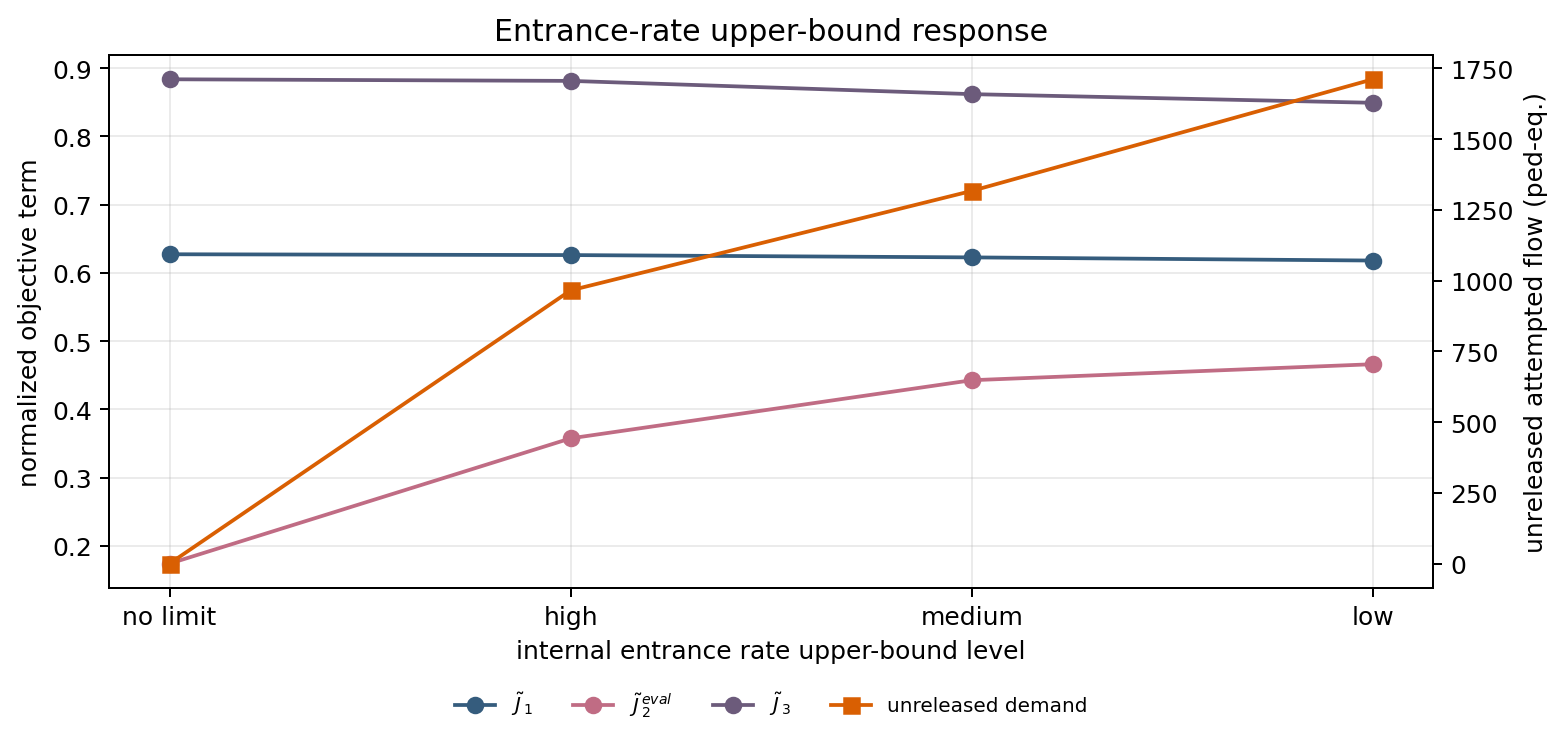
\includegraphics[width=\columnwidth]{figures/g2_capacity_levels.png}
\figcaptiontight
\caption{Objective-term response under internal entrance-rate upper-bound levels. Tightening the upper bound changes safety exposure, load balance, and unreleased attempted flow; the latter is reported in pedestrian-equivalent demand (ped-eq.).}
\label{fig:entrance_rate_response}
\end{figure}

Table~\ref{tab:entrance_rate_response} and Fig.~\ref{fig:entrance_rate_response} show that tightening the rate upper bound does not simply improve safety.
From the no-limit case to the low level, unreleased attempted flow increases from $0$ to $1.71\times10^{3}$~ped-eq., corresponding to $r_{\mathrm{rel}}=92.1\%$ of attempted entrance demand.
The binding ratio increases from $0$ to $0.721$, and the scaled normalized safety term $\tilde J_2$ increases from $0.174$ to $0.466$.
Thus, $q$ is a genuine continuous control variable that changes system response and must be optimized jointly with $s$.

\subsection{Horizontal Optimization Comparison}
\label{sec:optimal}

The horizontal comparison evaluates Prior Baseline, Random Search, Pure Simulated Annealing (Pure SA), Enumeration plus Differential Evolution (Enum-DE), TPE-Mixed BO, and HCMBO.
All optimizers use $B=400$ candidate evaluations and top-$10$ high-fidelity rechecks over seeds $11$, $23$, $37$, $51$, and $73$.


\begin{table}[!t]
\centering
\caption{High-Fidelity Performance Under the Full Five-Term Dimensionless Objective}
\label{tab:optimizer_summary}
\footnotesize
\setlength{\tabcolsep}{2pt}
\begin{tabular}{@{}>{\raggedright\arraybackslash}p{0.20\columnwidth}r r r r r >{\centering\arraybackslash}p{0.13\columnwidth}@{}}
\hline
Method & Mean objective & Std. & Median & Best & Worst & Feasible rate \\
\hline
HCMBO & \textbf{2.6338} & 0.3106 & \textbf{2.5065} & \textbf{2.4495} & 3.1851 & \textbf{100\%} \\
TPE-Mixed BO & 2.7403 & 0.2475 & 2.6288 & 2.5180 & 3.1345 & 80\% \\
Pure SA & 2.9248 & 0.1386 & 2.9203 & 2.7468 & 3.1049 & 60\% \\
Random Search & 3.0112 & 0.1319 & 2.9797 & 2.8821 & 3.2287 & 40\% \\
Enum-DE & 3.0597 & 0.1932 & 3.1004 & 2.7329 & 3.2500 & 40\% \\
Prior Baseline & 5.4774 & 0.0000 & 5.4774 & 5.4774 & 5.4774 & 0\% \\
\hline
\end{tabular}
\par\vspace{3.5mm}
\noindent\parbox{\columnwidth}{\footnotesize The reported objective is the full dimensionless scalar objective $J=\sum_{k=1}^{5}\lambda_k\tilde J_k$ after unified high-fidelity rechecking. These values are not directly comparable with the reduced diagnostic objective $J^{(3)}$ in Tables~\ref{tab:g2_nondominated}, \ref{tab:entrance_rate_response}, and \ref{tab:bund_transfer_metrics}.}
\end{table}

Table~\ref{tab:optimizer_summary} reports the smallest mean, median, and best objective for HCMBO, together with the highest feasible rate among the tested methods.
Its mean objective is $3.9\%$ lower than TPE-Mixed BO, since $(2.7403-2.6338)/2.7403=3.9\%$.
Because this is a normalized scalar objective, the percentage reduction reflects the fixed-weight management score, not a direct reduction in travel time or density exposure alone.
In paired comparisons, HCMBO has a lower objective than TPE-Mixed BO in four of five seeds, with an average objective difference of $-0.1066$.
It is also lower than Random Search in all five seeds and lower than Pure SA and Enum-DE in four of five seeds.
The remaining high HCMBO objective is mainly caused by a larger safety-exposure term, so later versions should add more explicit safety constraints during search.

\begin{figure}[!t]
\centering
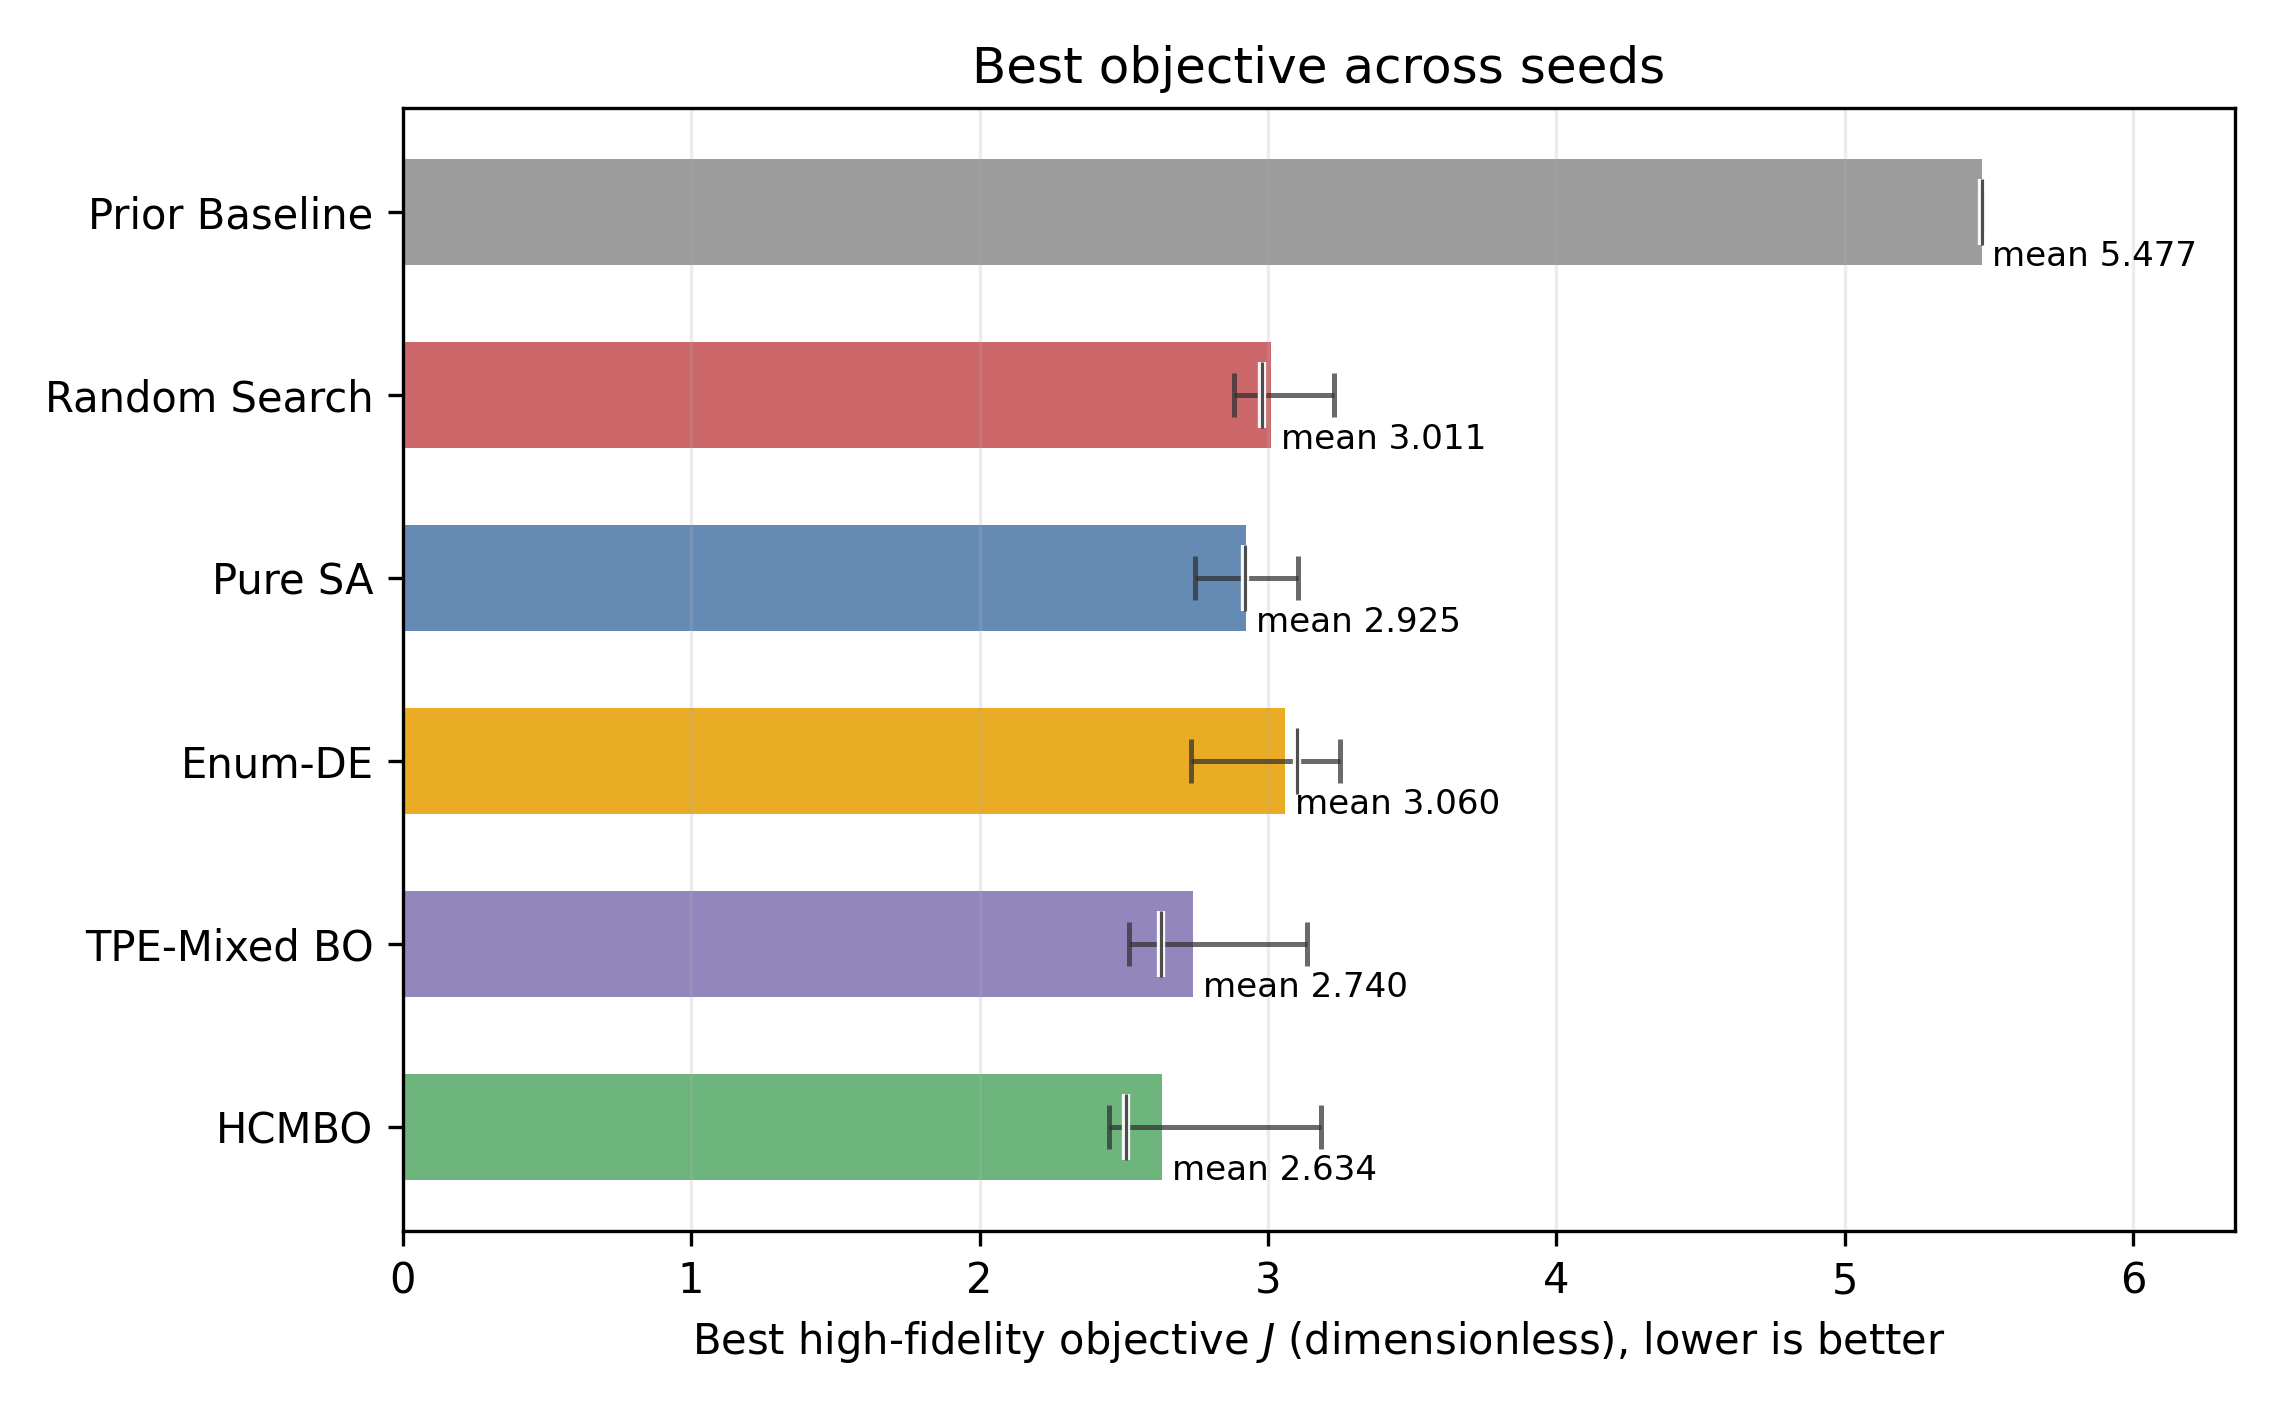
\includegraphics[width=\columnwidth]{figures/hcmbo_best_objective.png}
\figcaptiontight
\caption{Best high-fidelity full objective $J$ across seeds. The objective is dimensionless and lower is better. Range bars show the seed-wise spread, and the short vertical mark indicates the median.}
\label{fig:optimizer_best_objective}
\end{figure}

\begin{figure}[!t]
\centering
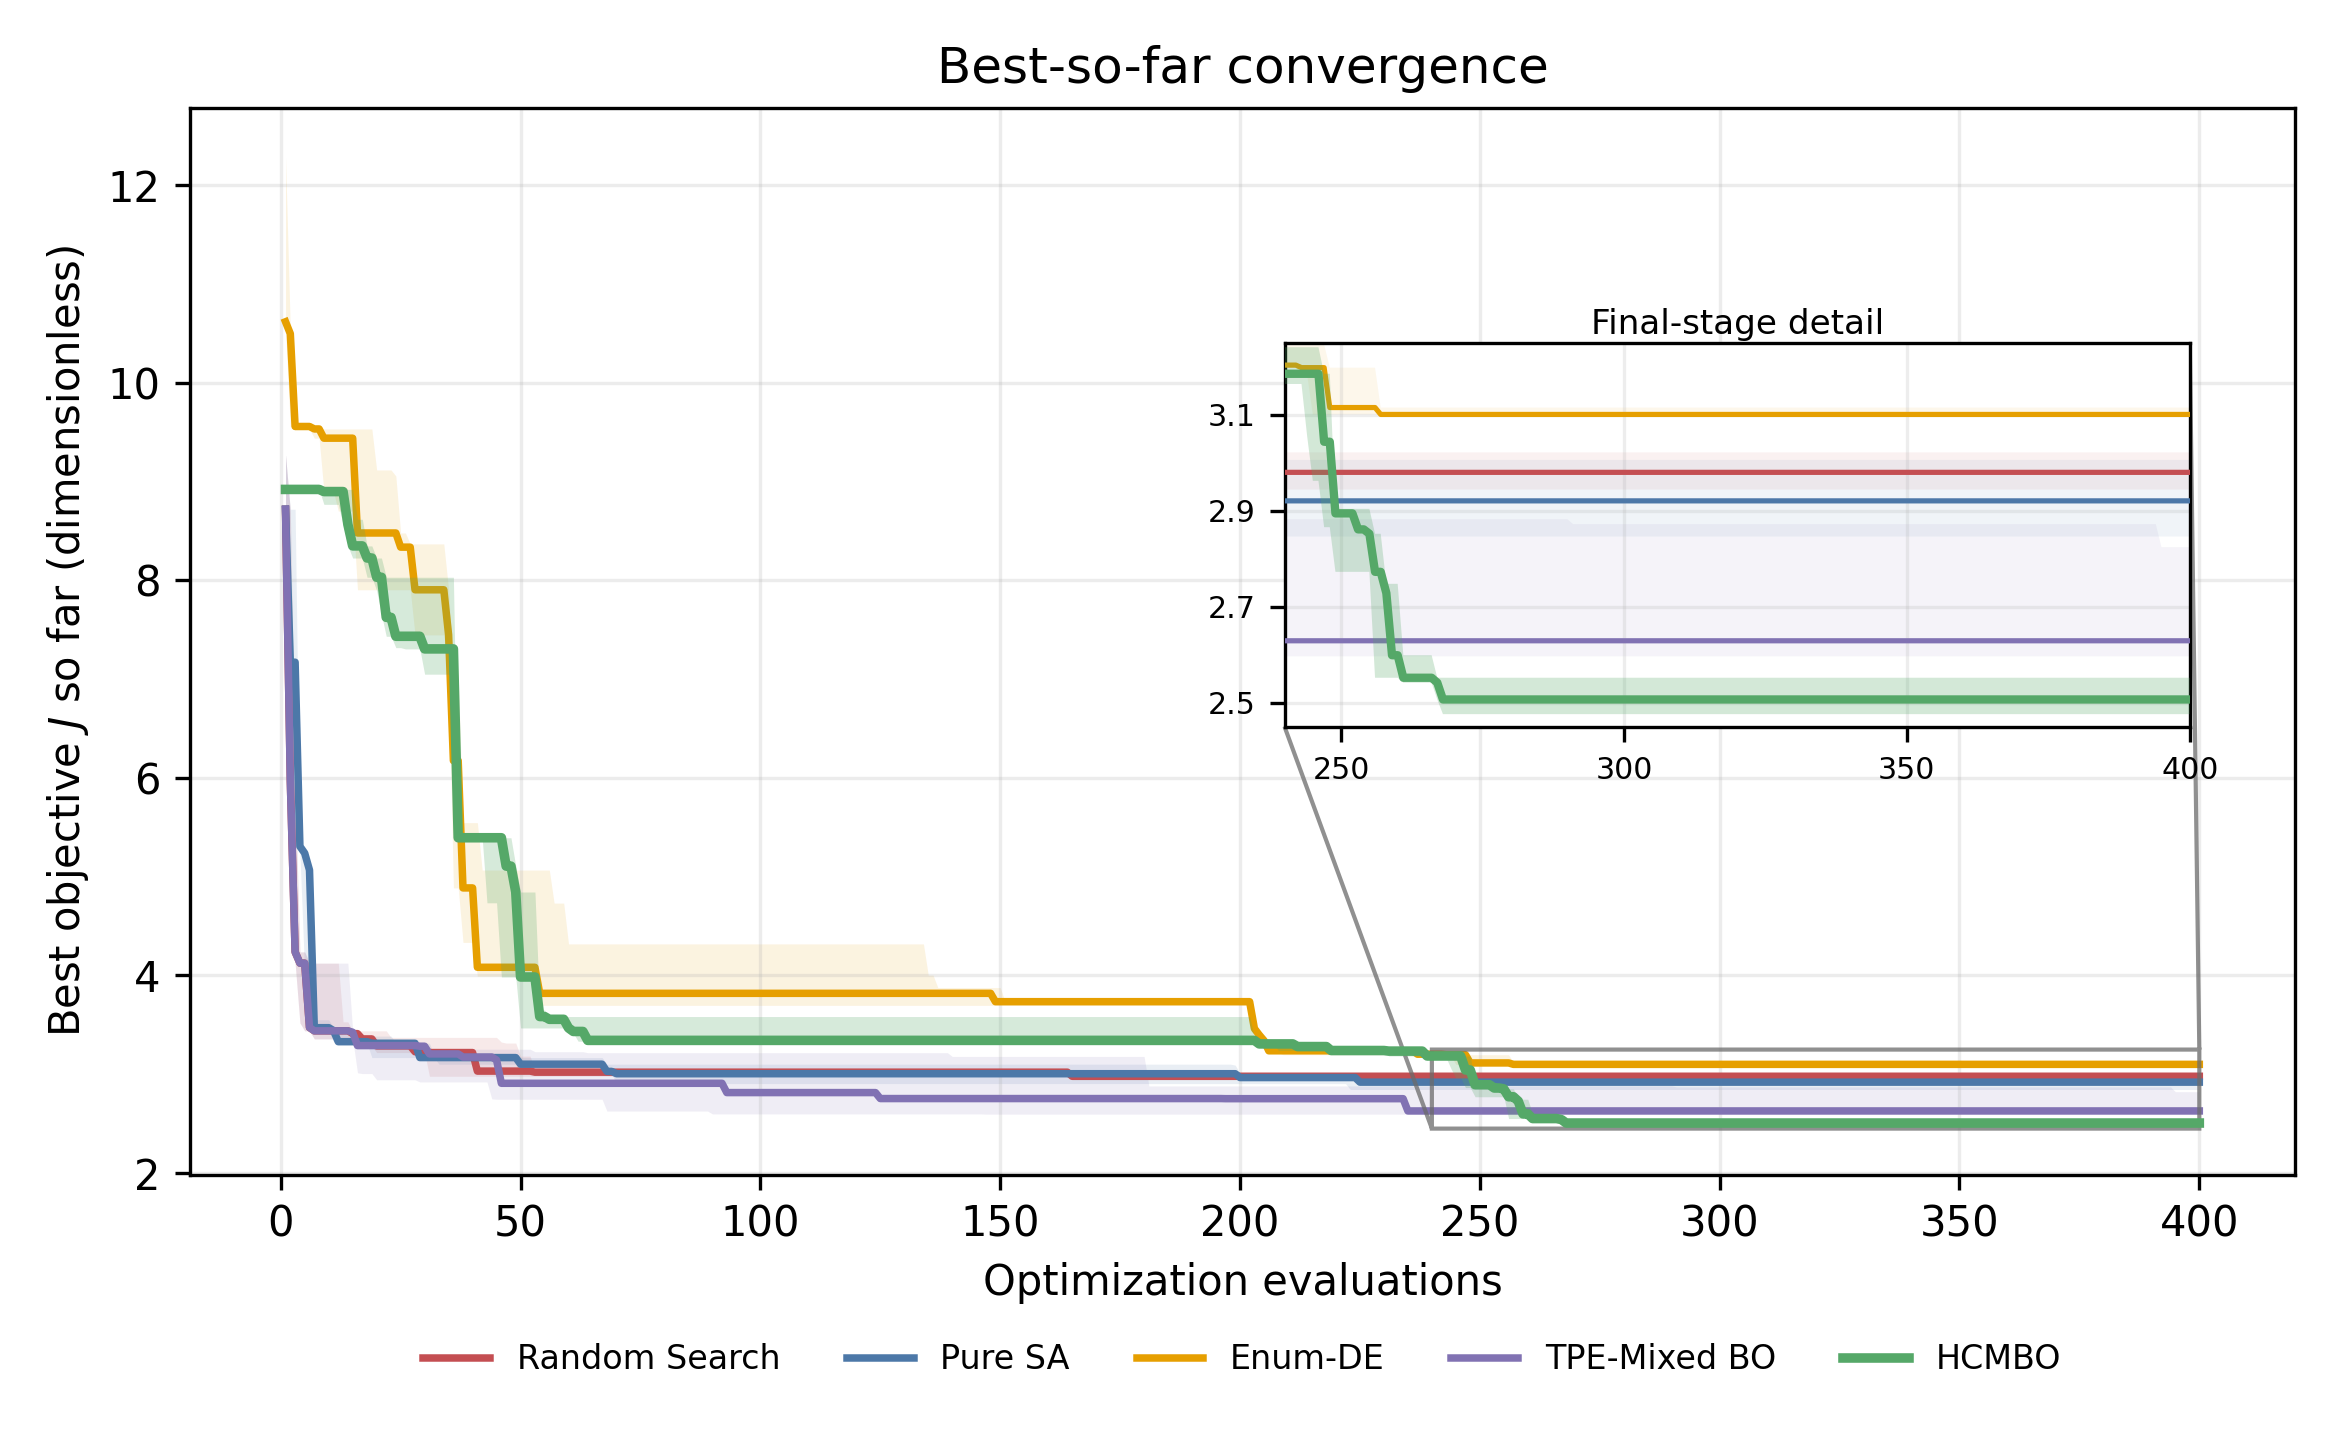
\includegraphics[width=\columnwidth]{figures/hcmbo_convergence.png}
\figcaptiontight
\caption{Best-so-far convergence curves under the same $400$-evaluation budget. The inset highlights the final-stage separation among methods.}
\label{fig:optimizer_convergence}
\end{figure}

\begin{figure}[!t]
\centering
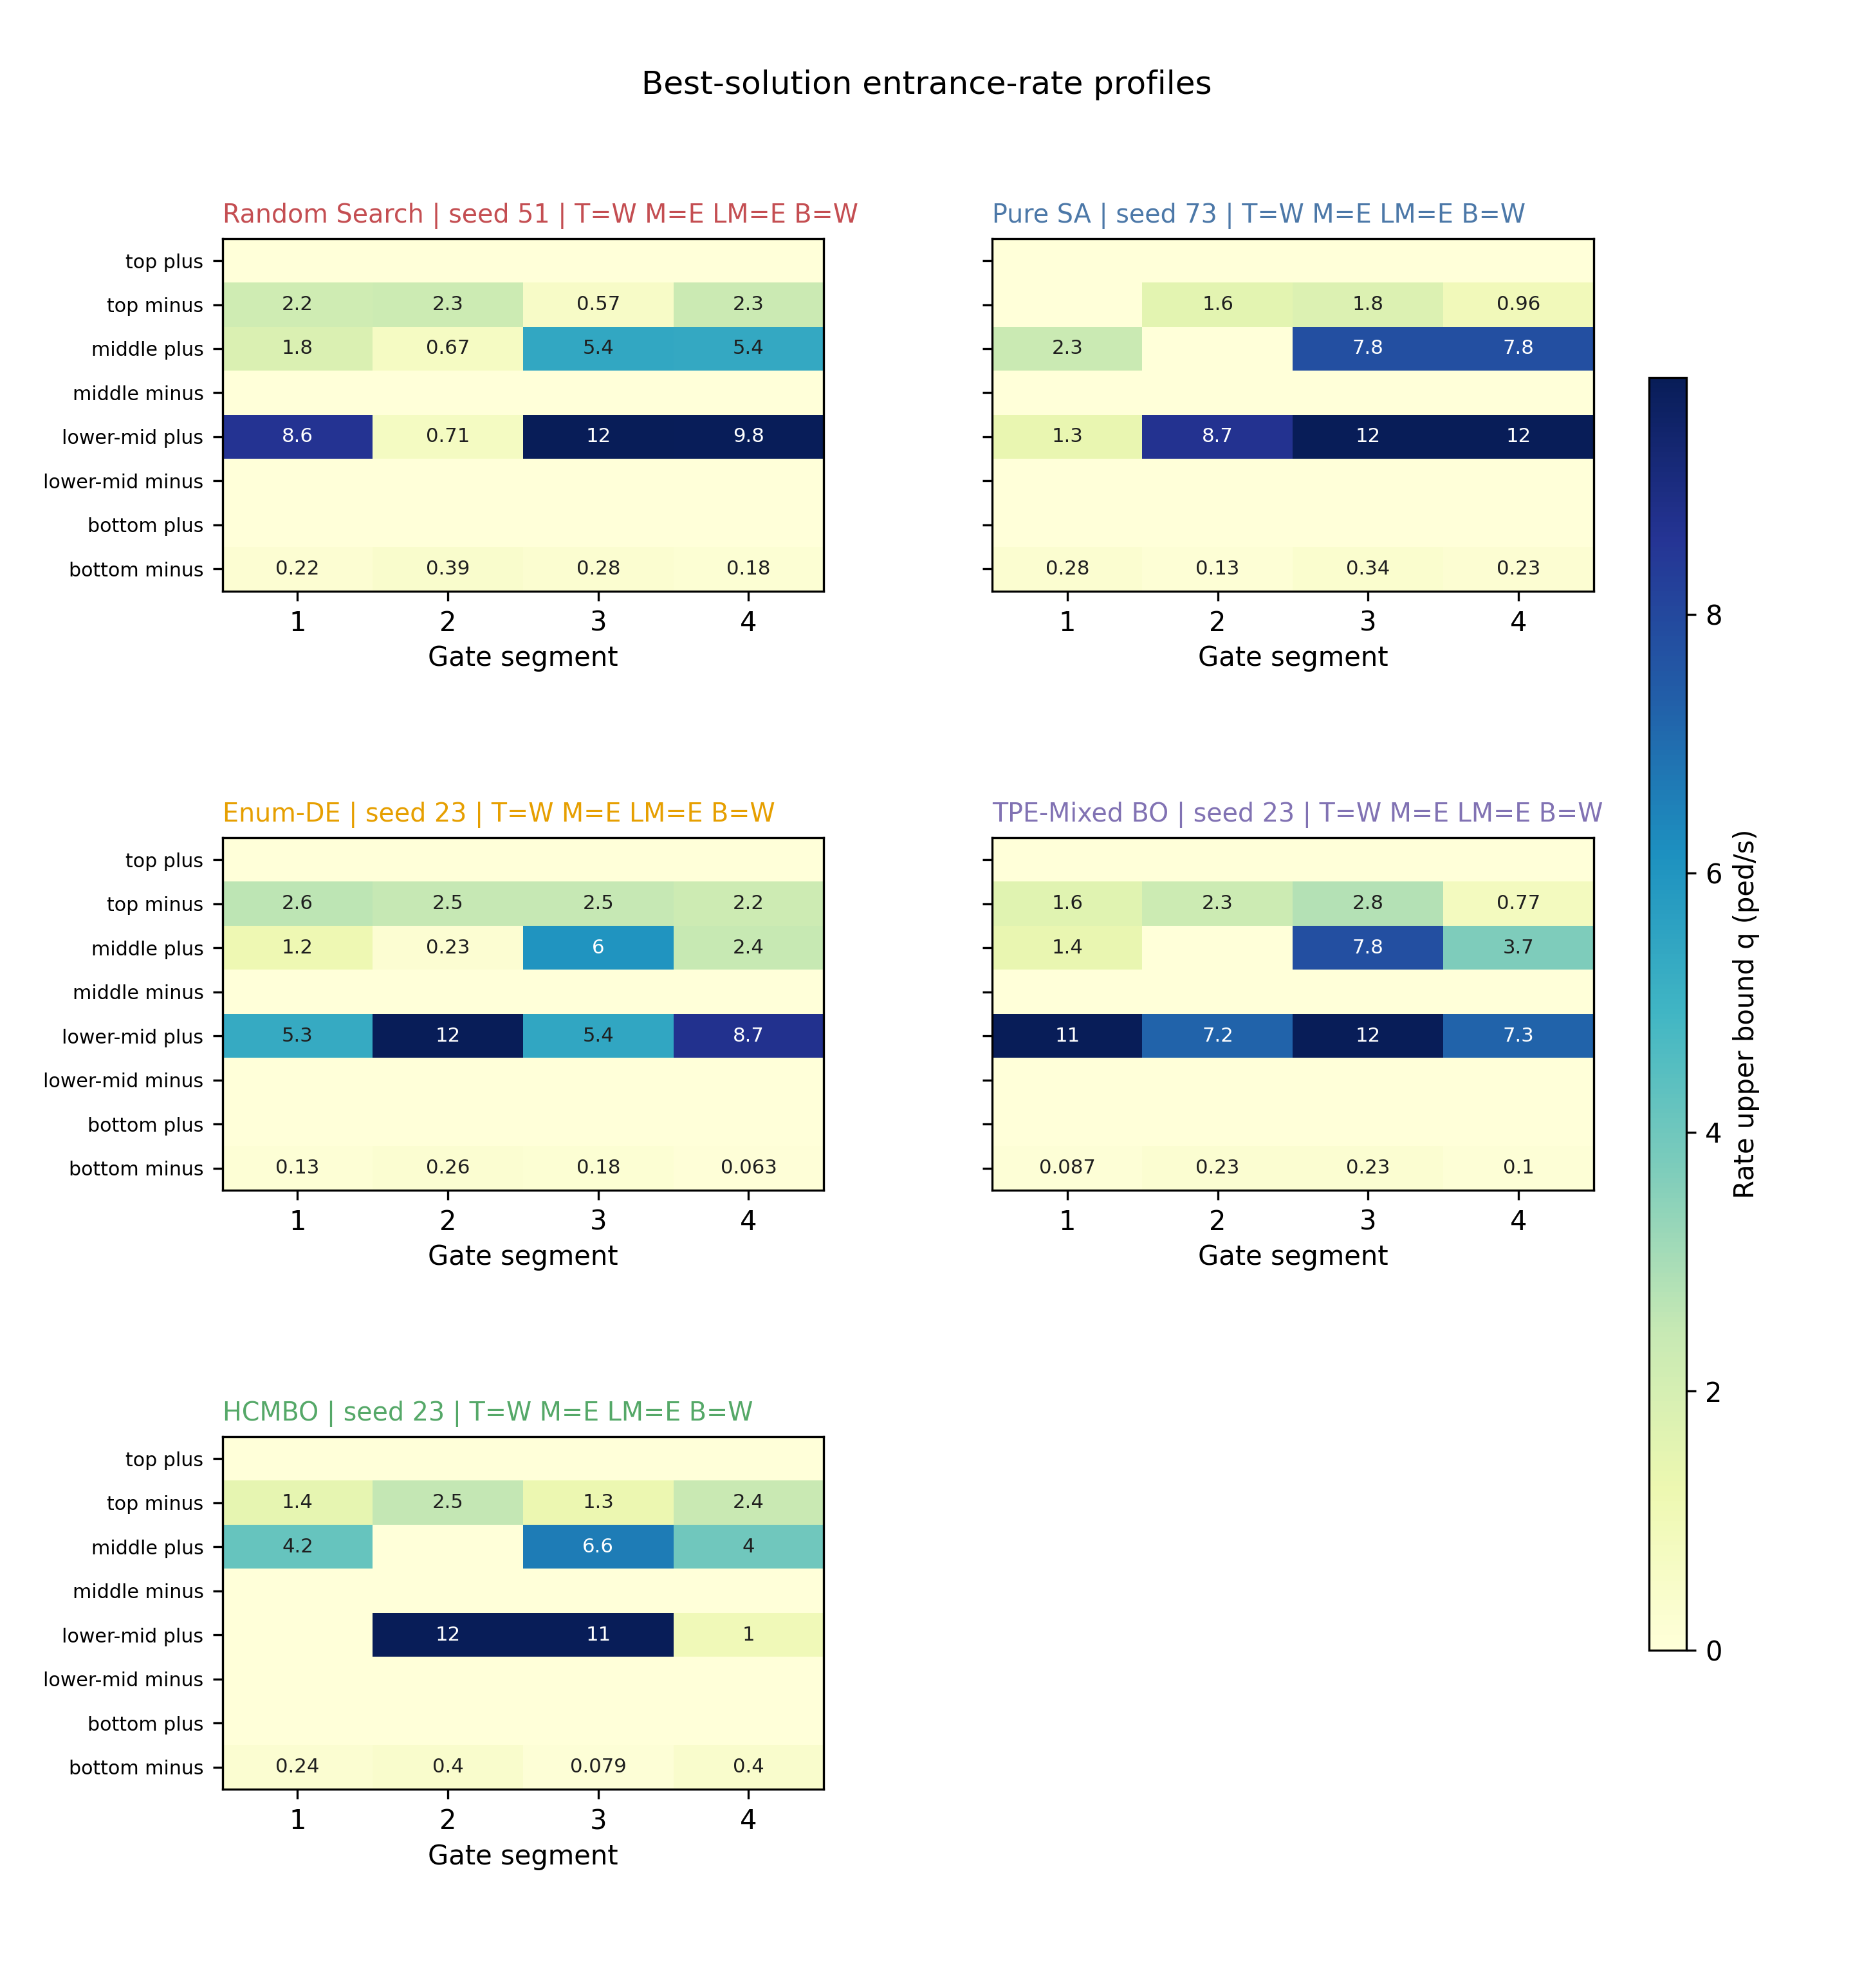
\includegraphics[width=\columnwidth]{figures/hcmbo_control_profiles.png}
\figcaptiontight
\caption{Best-solution entrance-rate profiles for Random Search, Pure SA, Enum-DE, TPE-Mixed BO, and HCMBO. The common direction structure is $[T,M,LM,B]=[W,E,E,W]$ for several methods, but the segment-wise rate allocations differ substantially.}
\label{fig:control_profiles}
\end{figure}

Figs.~\ref{fig:optimizer_best_objective}--\ref{fig:control_profiles} compare the seed-wise objectives, convergence traces, and selected entrance-rate profiles.
TPE-Mixed BO decreases quickly in the early evaluations, whereas HCMBO continues to reduce the best-so-far objective during the middle and late stages.
The control profiles indicate that methods with the same direction code can still choose different segment-wise rate allocations, leading to different final objectives.

\subsection{HCMBO Ablation}
\label{sec:ablation}

The ablation experiments test the contribution of each control and search component.
Optimizing only directions with a fixed high rate gives a best high-fidelity objective of $3.3751$, and optimizing only rates under prior directions gives $3.3140$; both are higher than the joint optimization result.
Short-horizon low-fidelity hard screening raises the best objective to $2.9441$ and selects an infeasible best candidate, because early simulations do not reliably capture long-horizon entrance waiting and load redistribution.
Removing the entrance-waiting penalty slightly lowers the scalar objective to $2.6015$, but increases unreleased attempted flow to approximately $1.30\times10^4$~ped-eq.
The waiting term should therefore remain in the management objective.
In the search-mechanism variants, lower confidence bound (LCB) denotes the acquisition rule, and random-forest-style (RF-style) denotes the constrained Bayesian-optimization surrogate variant.

\begin{table}[!t]
\centering
\caption{Search-Mechanism Ablation Under Seed 23}
\label{tab:search_ablation}
\footnotesize
\setlength{\tabcolsep}{1pt}
\makebox[\columnwidth][c]{%
\renewcommand{\arraystretch}{1.12}%
\setlength{\extrarowheight}{0.6pt}%
\begin{tabular}{@{}>{\raggedright\arraybackslash}m{0.22\columnwidth}
>{\centering\arraybackslash}m{0.12\columnwidth}
>{\centering\arraybackslash}m{0.11\columnwidth}
>{\centering\arraybackslash}m{0.10\columnwidth}
>{\centering\arraybackslash}m{0.16\columnwidth}
>{\raggedright\arraybackslash}m{0.23\columnwidth}@{}}
\hline
Variant & Best objective & Feasible rate & $\tilde J_2$ & Unreleased flow (ped-eq.) & Main meaning \\
\hline
HCMBO & \textbf{2.4495} & 100\% & \textbf{1.6759} & $1.02{\times}10^4$ & Structured direction-wise rate search \\
Queue-aware LCB & 2.6162 & 100\% & 1.8521 & $\mathbf{9.64{\times}10^3}$ & Queue-aware acquisition \\
RF-style constrained BO & 2.6162 & 100\% & 1.8521 & $\mathbf{9.64{\times}10^3}$ & Constraint surrogate variant \\
Adaptive racing & 2.6561 & 100\% & 1.9474 & $1.28{\times}10^4$ & Stage-wise budget concentration \\
Adaptive racing + queue-aware & 2.6683 & 100\% & 1.7862 & $1.06{\times}10^4$ & Combined racing and queue signal \\
Trust-region search & 3.0317 & 100\% & 1.9224 & $1.59{\times}10^4$ & Local trust-region search \\
\hline
\end{tabular}
}
\par\vspace{3.5mm}
\noindent\parbox{\columnwidth}{\footnotesize Unreleased flow is the cumulative unreleased attempted entrance flow over the full horizon, in pedestrian-equivalent demand (ped-eq.); it integrates repeatedly denied demand and is not an instantaneous queue length.}
\end{table}

Table~\ref{tab:search_ablation} shows that the final HCMBO mainline has the lowest scalar objective among the tested variants.
Queue-aware LCB and RF-style constrained BO reduce unreleased attempted flow to approximately $9.64\times10^3$~ped-eq., but their scalar objective increases to $2.6162$.
Thus, queue information is useful for executable and safety-aware extensions, whereas the final mainline should retain structured direction-wise rate search as the primary budget allocation mechanism.

\subsection{Transfer Validation on a Bund-Inspired Scenario}
\label{sec:bund_transfer}

The preceding experiments use a standardized four-channel platform scenario to verify modeling mechanisms and optimization behavior under controlled conditions.
As a supplementary validation, we further construct a simplified abstract scenario inspired by the spatial form of the Shanghai Bund waterfront.
This experiment does not claim to reproduce all architectural details of the real site.
Instead, it preserves the Bund sightseeing platform, the lateral passage connections, the major inflow location, and the dominant movement direction, so as to examine whether an HCMBO-derived policy can still change the load distribution in a more realistic spatial outline.

\begin{figure*}[!t]
\centering
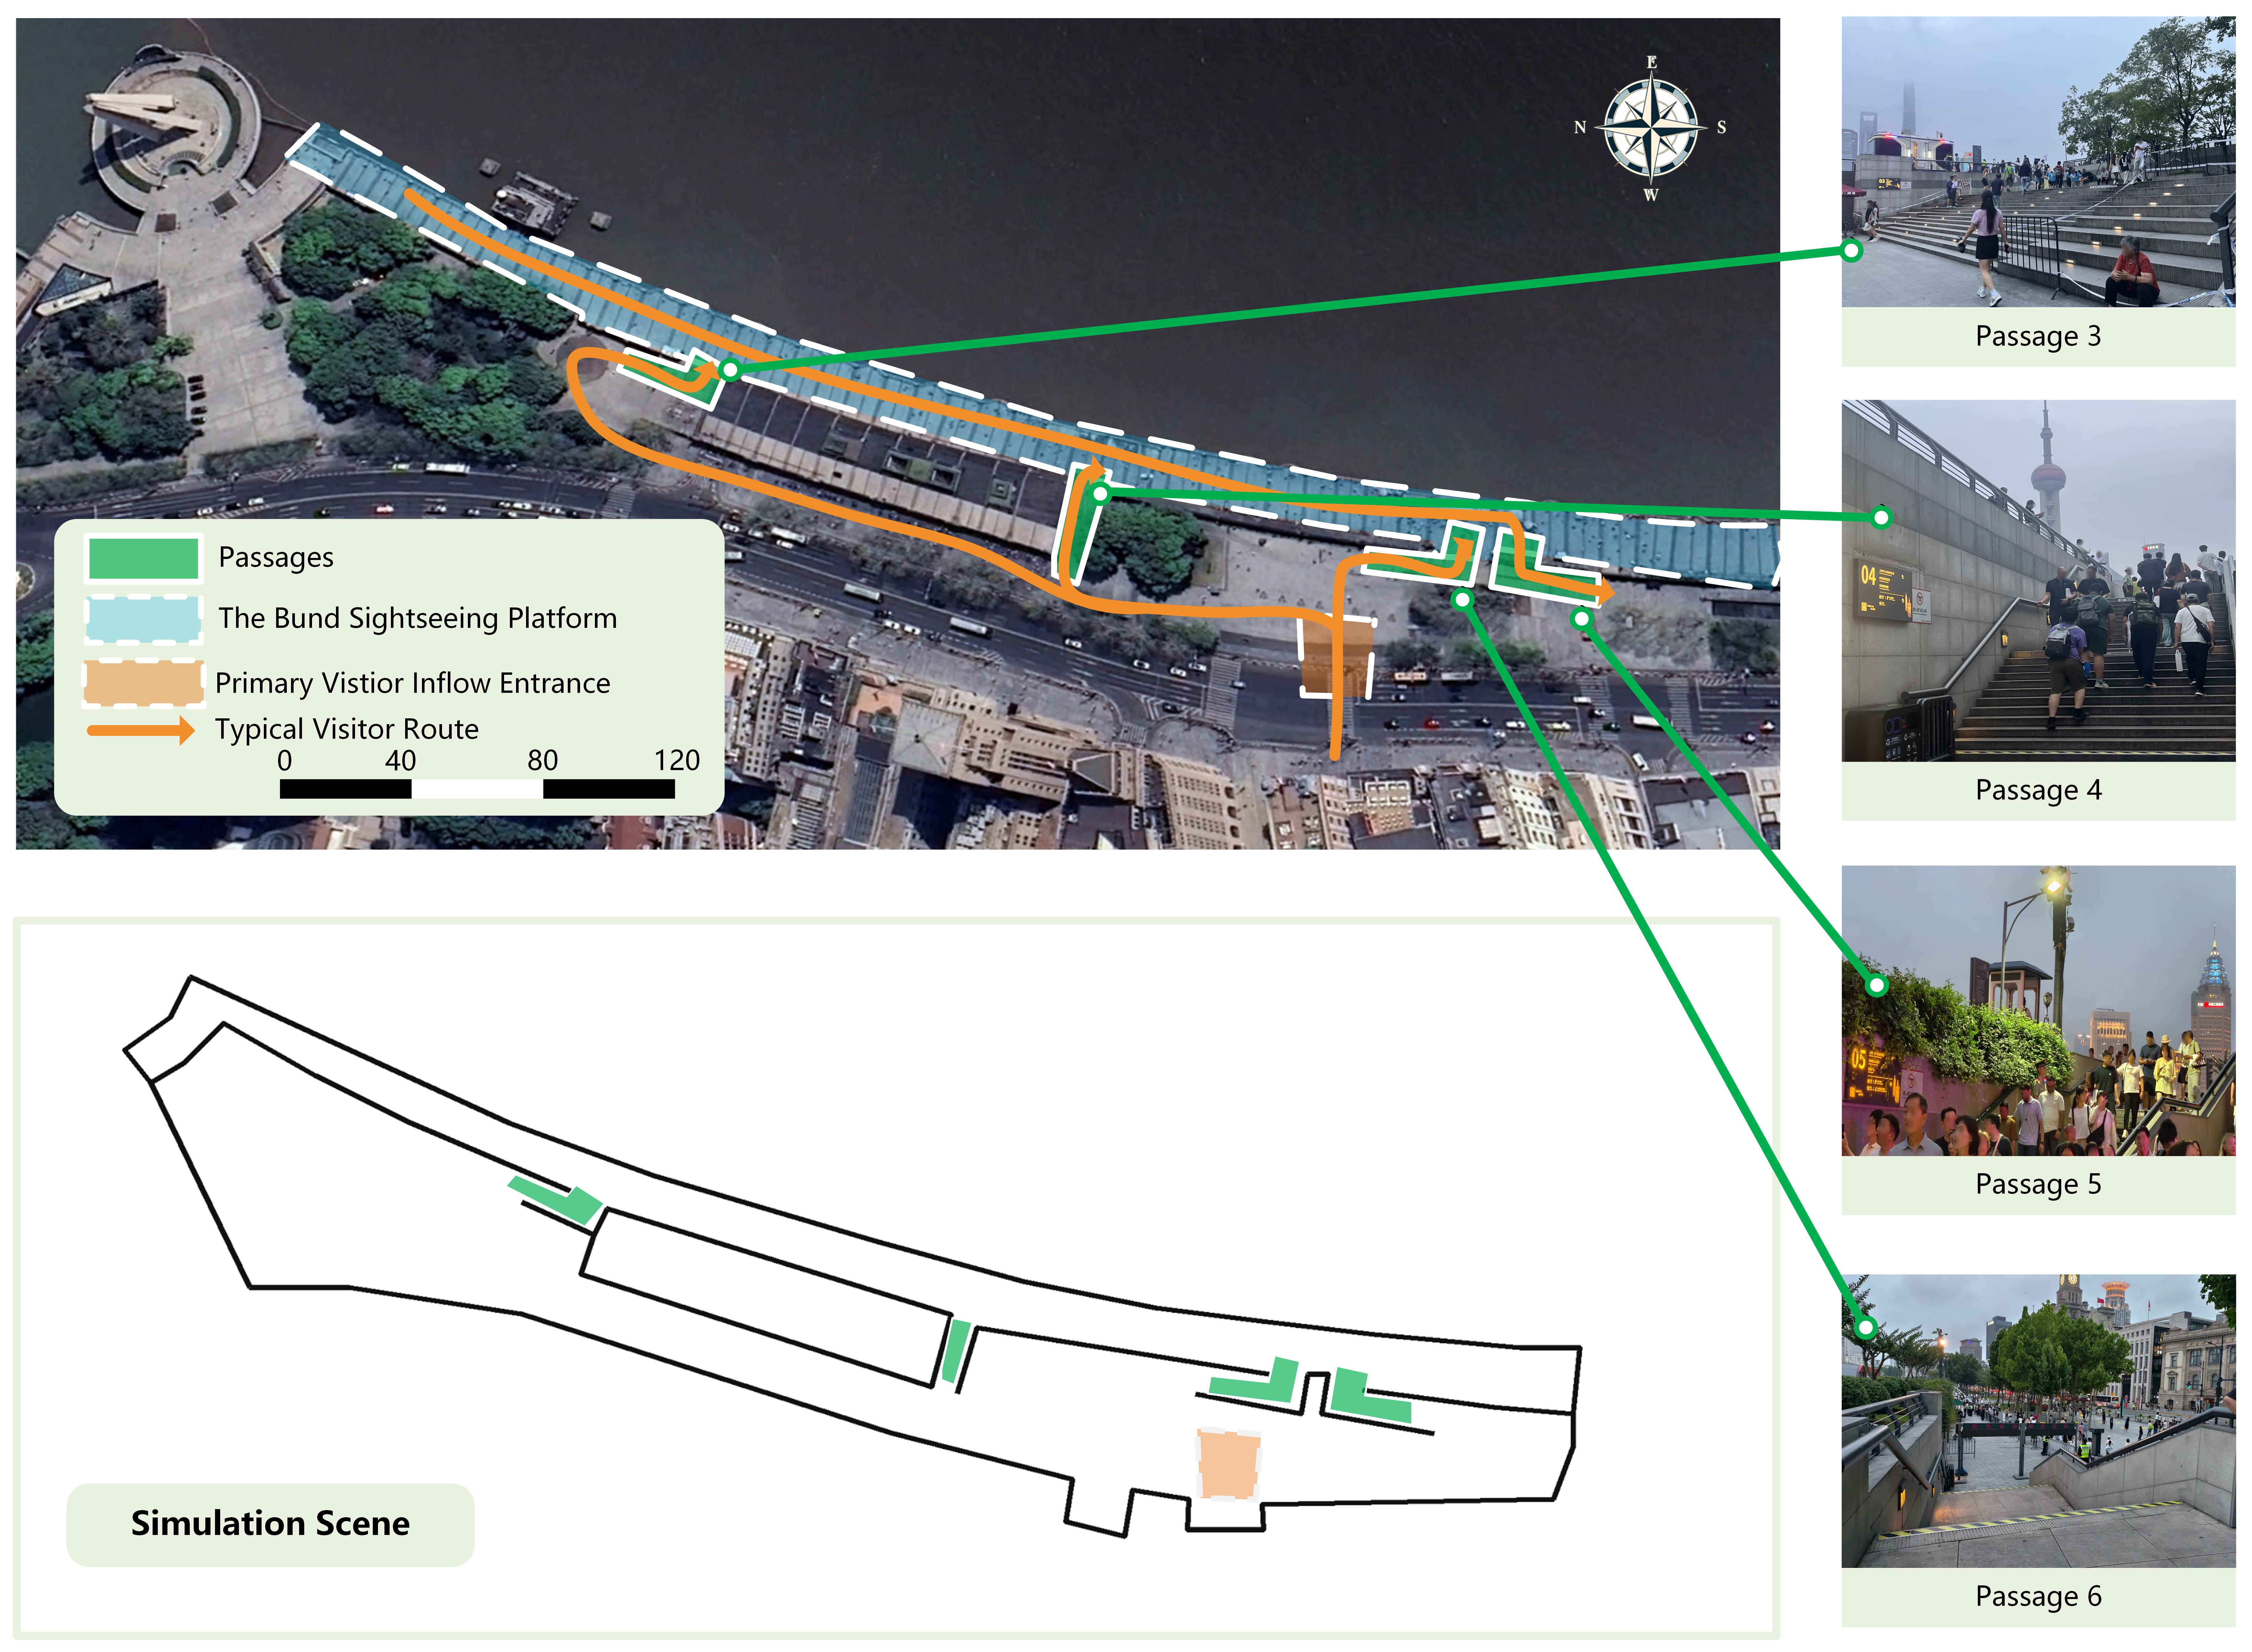
\includegraphics[width=0.82\textwidth]{figures/bund_scene_schematic.jpg}
\figcaptiontight
\caption{Real Bund scene and its simplified simulation abstraction. The abstraction retains the Bund sightseeing platform boundary, the main entrance, and the passage connections used for control validation. The satellite basemap was obtained from Google Maps. The right-side local photographs were shot in the Shanghai Bund waterfront passage area by the Tongji Public Safety Experimental Team, June 21, 2026.}
\label{fig:bund_transfer_scene}
\end{figure*}

The computational grid has resolution $512\times224$.
Because this scenario preserves the real Bund outline, its physical scale is calibrated from georeferenced control points that match the scene coordinates to satellite latitude and longitude; a four-point affine fit gives $0.435$~m per scene unit with sub-$1.5$~m residual, which corresponds to a physical cell size of about $1.75$~m.
The $512\times224$ grid therefore spans approximately $894~\mathrm{m}\times391~\mathrm{m}$, the induced time step is $\Delta t\approx0.44$~s, and pedestrian counts again follow by integrating density over physical area (a cell area of about $3.0$~m$^2$).
Pedestrians enter from the outer-side entrance, pass through the middle connecting channels, and move toward the Bund sightseeing platform and its central target region.
The inflow-rate multiplier is $3.0$, corresponding to an actual inflow rate of about $3.35$~ped/s; the maximum density is $\rho_{\max}=4.0$~ped/m$^2$, and the stage-switching rate is $\kappa_{\sigma,r}=32$ in simulation time units.
The experimental channels \texttt{channel\_1}, \texttt{channel\_2}, \texttt{channel\_3}, and \texttt{channel\_4} correspond to the locally named Bund Passages 3, 4, 5, and 6, respectively.
Both the controlled and uncontrolled groups use $1600$ steps over a physical horizon of about $698$~s.
For the controlled group, the transferred entrance-rate bounds are multiplied by a capacity-scale factor of $3$, providing a less restrictive entrance-capacity setting.

The controlled group uses the best HCMBO policy obtained from the multi-direction high-fidelity recheck.
Its reduced high-fidelity objective in the optimization stage is $0.7350$, and its direction structure leaves the upper and lower channels bidirectional while assigning opposite dominant directions to the two middle channels.
Table~\ref{tab:bund_transfer_q} reports the effective two-segment entrance-rate upper bounds after applying the capacity-scale factor of $3$.
The rate upper bounds are measured in ped/s.

\begin{table}[!t]
\centering
\caption{Effective Entrance-Rate Upper Bounds in the Bund Transfer Experiment}
\label{tab:bund_transfer_q}
\footnotesize
\setlength{\tabcolsep}{1pt}
\begin{tabular}{@{}>{\raggedright\arraybackslash}p{0.23\columnwidth}
>{\raggedright\arraybackslash}p{0.18\columnwidth}
>{\raggedright\arraybackslash}p{0.18\columnwidth}
>{\centering\arraybackslash}p{0.16\columnwidth}
>{\centering\arraybackslash}p{0.16\columnwidth}@{}}
\hline
Experimental channel & Local passage name & Entrance side & Segment 1 (ped/s) & Segment 2 (ped/s) \\
\hline
\texttt{channel\_1} & Bund Passage 3 & Forward entrance & 3.45 & 8.38 \\
\texttt{channel\_1} & Bund Passage 3 & Reverse entrance & 3.17 & 0.00 \\
\texttt{channel\_2} & Bund Passage 4 & Forward entrance & 8.38 & 2.36 \\
\texttt{channel\_2} & Bund Passage 4 & Reverse entrance & 0.00 & 0.00 \\
\texttt{channel\_3} & Bund Passage 5 & Forward entrance & 0.00 & 0.00 \\
\texttt{channel\_3} & Bund Passage 5 & Reverse entrance & 3.57 & 6.95 \\
\texttt{channel\_4} & Bund Passage 6 & Forward entrance & 5.28 & 3.03 \\
\texttt{channel\_4} & Bund Passage 6 & Reverse entrance & 3.09 & 2.96 \\
\hline
\end{tabular}
\end{table}

Table~\ref{tab:bund_transfer_metrics} compares the controlled and uncontrolled groups under the same high-fidelity protocol.
It separates dimensionless normalized terms from raw simulation diagnostics.
The reduced objective $J^{(3)}$ decreases from $1.0140$ to $0.7410$, corresponding to an absolute reduction of approximately $0.2730$ and a relative reduction of $26.9\%$.
The largest reduction comes from the load-balance term $\tilde J_3$, which decreases by $51.9\%$, from $0.6043$ to $0.2908$.
In contrast, $\tilde J_1$ increases by $8.7\%$ and $\tilde J_2$ increases by $25.7\%$.
This indicates that the transferred policy changes how pedestrians use the channels, rather than merely reducing all density values uniformly.

\begin{table}[!t]
\centering
\caption{Controlled and Uncontrolled Results in the Bund Transfer Experiment}
\label{tab:bund_transfer_metrics}
\footnotesize
\setlength{\tabcolsep}{2pt}
\begin{tabular}{@{}>{\raggedright\arraybackslash}p{0.35\columnwidth}r r r@{}}
\hline
Dimensionless term & Controlled & Uncontrolled & Relative change \\
\hline
$J^{(3)}$ & 0.7410 & 1.0140 & $-26.9\%$ \\
$\tilde J_1$ & 0.4145 & 0.3813 & $+8.7\%$ \\
$\tilde J_2$ & 0.0357 & 0.0284 & $+25.7\%$ \\
$\tilde J_3$ & 0.2908 & 0.6043 & $-51.9\%$ \\
\hline
\end{tabular}

\vspace{1.5mm}
\begin{tabular}{@{}>{\raggedright\arraybackslash}p{0.43\columnwidth}c c l@{}}
\hline
Raw diagnostic & Controlled & Uncontrolled & Unit \\
\hline
Final cumulative sink flow & $1.33{\times}10^3$ & $1.67{\times}10^3$ & ped \\
Final cumulative inflow & $2.32{\times}10^3$ & $2.34{\times}10^3$ & ped \\
Final system mass & $1.53{\times}10^3$ & $1.20{\times}10^3$ & ped \\
Peak density maximum & $\approx 4.0$ & $\approx 4.0$ & ped/m$^2$ \\
Domain-mean density (incl. empty space) & $3.47{\times}10^{-3}$ & $3.21{\times}10^{-3}$ & ped/m$^2$ \\
Attempted entrance flow & $1.49{\times}10^3$ & \multicolumn{1}{c}{--} & ped-eq. \\
Actual entrance flow & $1.13{\times}10^3$ & \multicolumn{1}{c}{--} & ped \\
Unreleased attempted flow & $364$ & \multicolumn{1}{c}{--} & ped-eq. \\
\hline
\end{tabular}

\par\vspace{3.5mm}
\noindent\parbox{\columnwidth}{\footnotesize Sink flow, inflow, system mass, and actual entrance flow are pedestrian counts (ped). Attempted and unreleased entrance flow are cumulative pedestrian-equivalent demand (ped-eq.): they integrate repeatedly denied demand over the horizon and may exceed the number of distinct waiting pedestrians. Entries marked $-$ are not applicable because the uncontrolled case activates no internal metering interface. The domain-mean density is averaged over the full walkable domain, including empty space, and is therefore much smaller than the local peak.}
\end{table}

The channel-flow shares in Table~\ref{tab:bund_transfer_flux} further explain this reduction.
In the uncontrolled group, $82.30\%$ of the channel flow concentrates on \texttt{channel\_4}, i.e., Bund Passage 6.
After applying the HCMBO policy, the flow is redistributed mainly to \texttt{channel\_2} and \texttt{channel\_3}, whose combined share reaches approximately $91.34\%$.

\begin{table}[!t]
\centering
\caption{Channel-Flow Shares in the Bund Transfer Experiment}
\label{tab:bund_transfer_flux}
\footnotesize
\setlength{\tabcolsep}{4pt}
\begin{tabular}{l l r r}
\hline
Channel & Local name & Controlled & Uncontrolled \\
\hline
\texttt{channel\_1} & Bund Passage 3 & 2.83\% & 0.32\% \\
\texttt{channel\_2} & Bund Passage 4 & 30.38\% & 1.35\% \\
\texttt{channel\_3} & Bund Passage 5 & 60.96\% & 16.03\% \\
\texttt{channel\_4} & Bund Passage 6 & 5.83\% & 82.30\% \\
\hline
\end{tabular}
\par\vspace{3.5mm}
\noindent\parbox{\columnwidth}{\footnotesize Channel-flow shares are computed as $R_c(T)/\sum_{j=1}^{C}R_j(T)$, where $R_c(T)$ is the realized cumulative admitted throughput of channel $c$ during the simulation horizon.}
\end{table}

\begin{figure*}[!t]
\centering
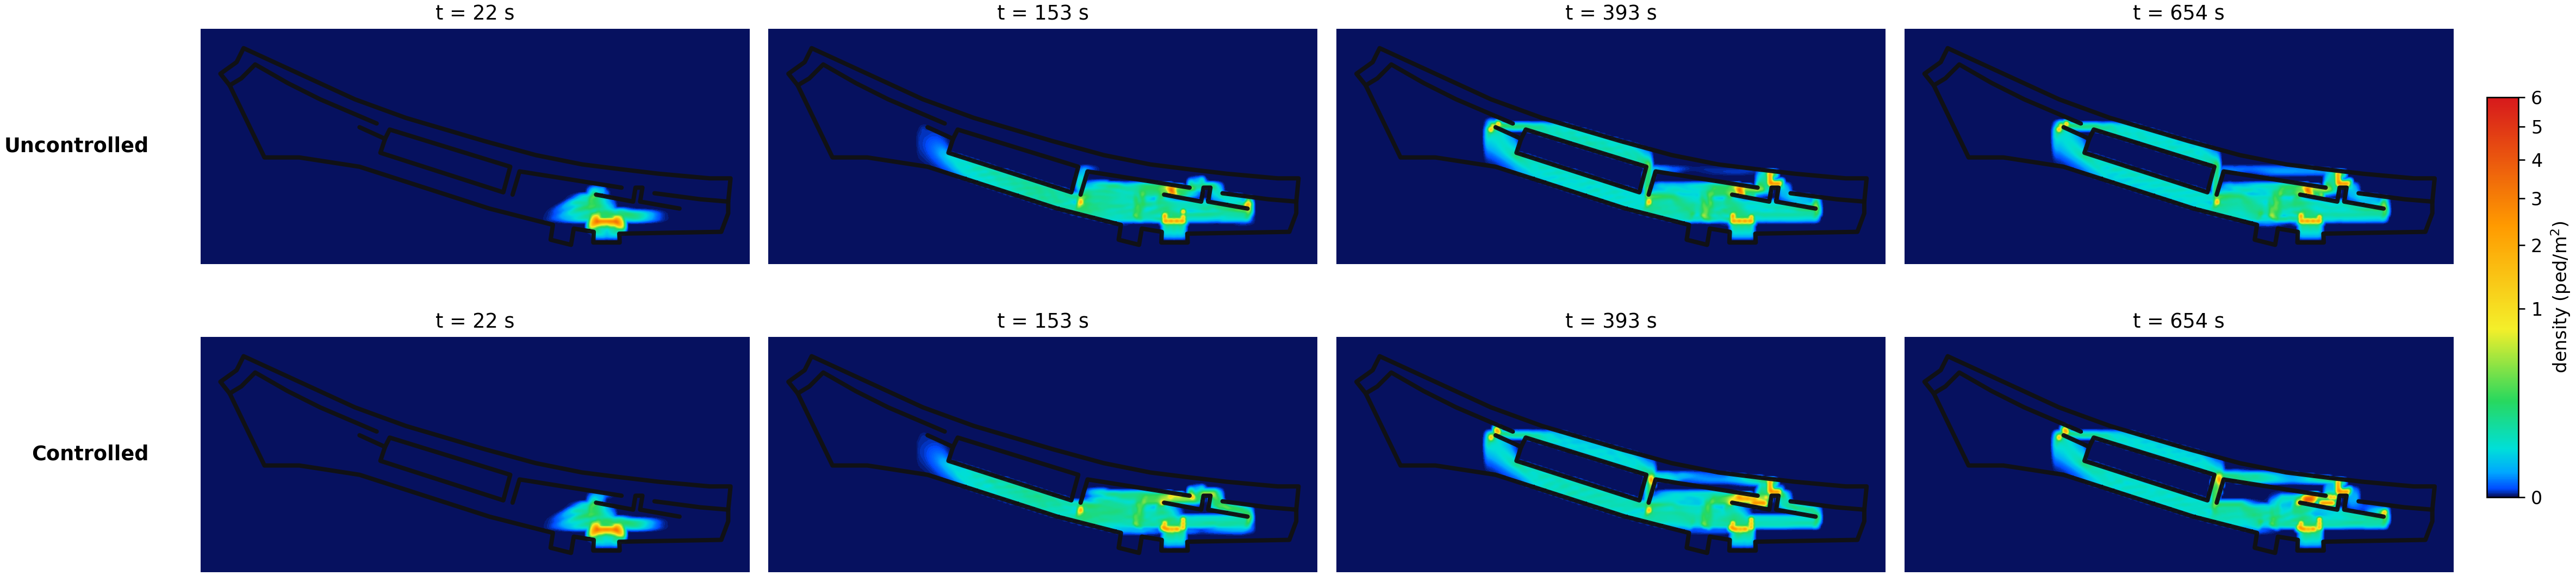
\includegraphics[width=0.95\textwidth]{figures/bund_density_panel.png}
\figcaptiontight
\caption{Density evolution comparison between uncontrolled and controlled cases at approximately $22$, $153$, $393$, and $654$~s. The controlled policy redistributes the later-stage flow from the terminal channel toward the middle-channel group.}
\label{fig:bund_transfer_density_panel}
\end{figure*}

Fig.~\ref{fig:bund_transfer_density_panel} visualizes the density evolution at approximately $22$, $153$, $393$, and $654$~s.
Both groups initially form a local density concentration near the right-side target region of the Bund sightseeing platform, reflecting the same inflow and target-attraction structure.
At later stages, the uncontrolled case remains more concentrated around the terminal channel and the adjacent Bund sightseeing platform area, whereas the controlled case develops a more stable flow band through the middle-channel group.
This visual evidence is consistent with the channel-share statistics and confirms that the main effect of the HCMBO policy is load redistribution across channels.

The transfer experiment exposes a trade-off.
Compared with the uncontrolled group, the controlled group has a higher efficiency term ($\tilde J_1$ increases from $0.3813$ to $0.4145$) and a slightly higher safety-exposure term ($\tilde J_2$ increases from $0.0284$ to $0.0357$).
Its cumulative sink flow is also smaller ($1.33{\times}10^3$ vs. $1.67{\times}10^3$~ped), and its final system mass is larger ($1.53{\times}10^3$ vs. $1.20{\times}10^3$~ped).
The transferred HCMBO policy therefore should not be read as a uniform safety or efficiency improvement.
Under the present reduced-objective weights, it lowers $J^{(3)}$ mainly by redistributing channel load, while giving up part of exit throughput and travel efficiency.
The capacity-scale factor of $3$ reduces unreleased attempted flow to $364$~ped-eq., but it does not remove the efficiency cost.
A deployment-oriented version should add explicit throughput constraints and waiting upper bounds, and should test several objective-weight settings before selecting a policy.

The real Bund waterfront operates at crowd scales far beyond the demonstration level of this section.
According to official holiday reports, the instantaneous on-site crowd in the Bund waterfront area peaked at $5.7\times10^4$ pedestrians during the 2025 National Day holiday \cite{qq2025bund_holiday_peak} and reached $7.1\times10^4$ during the 2019 holiday \cite{chinanews2019bund_flow_guidance}.
The present experiment deliberately adopts a lower demand setting so that the transfer of control mechanisms and optimized policies can be examined under controlled conditions, rather than reproducing peak holiday loads.

We emphasize that the computational cost of the macroscopic model is determined solely by the grid resolution and the number of simulation steps, and is independent of the number of pedestrians present: crowd size enters the model only through the magnitude of the density field and the entrance inflow rates.
Scaling from the demonstration level to a 50,000-pedestrian crowd-scale scenario therefore requires no change to the model structure, the numerical scheme, or the grid; only demand-side parameters change.
Table~\ref{tab:bund_scale_projection} contrasts the two crowd-scale scenarios.
The spatial extent, grid resolution, time step, and per-step cost are identical in both conditions; only the instantaneous population, the entrance inflow rates, and the horizon differ, and among these only the horizon increases the total cost, linearly in the number of steps.

\begin{table*}[!t]
\centering
\caption{Parameter Correspondence Between the Transfer Experiment and a Real-Scale Bund Crowd-scale Scenario}
\label{tab:bund_scale_projection}
\footnotesize
\setlength{\tabcolsep}{6pt}
\begin{tabular}{@{}>{\raggedright\arraybackslash}p{0.15\textwidth}
>{\raggedright\arraybackslash}p{0.26\textwidth}
>{\raggedright\arraybackslash}p{0.28\textwidth}
>{\raggedright\arraybackslash}p{0.24\textwidth}@{}}
\hline
Parameter & Transfer experiment & Real-scale scenario & Effect on cost \\
\hline
Spatial extent & $\approx894~\mathrm{m}\times391$~m (georeferenced) & identical (covers the waterfront core area) & unchanged \\
Grid resolution & $512\times224$, $\Delta x\approx1.75$~m & identical & sole spatial cost factor; unchanged \\
Time step & $\Delta t\approx0.44$~s (CFL-induced) & identical (independent of crowd size) & unchanged \\
Instantaneous population & peak $\approx1.5\times10^3$~ped & $5\times10^4$--$7\times10^4$~ped & none (density values only) \\
Peak local density & $\approx4.0$~ped/m$^2$ ($=\rho_{\max}$) & same saturated regime & none; regime already covered \\
Total entrance inflow & $\approx3.35$~ped/s (single main entrance) & $\approx20$--$30$~ped/s (multiple entrances, field-calibrated) & none (boundary condition) \\
Simulation horizon & $\approx698$~s ($1600$ steps) & $1$--$2$~h peak period ($\approx8\times10^3$--$1.6\times10^4$ steps) & total cost grows linearly with steps \\
\hline
\end{tabular}
\end{table*}

From a dynamics viewpoint, a crowd of $5\times10^4$--$7\times10^4$ pedestrians corresponds to an average walkable density of roughly $0.3$--$0.6$~ped/m$^2$, far below the jam density $\rho_{\max}=4.0$~ped/m$^2$, whereas the local peak density in this section already reaches $\rho_{\max}$; that is, the saturated congested branch of the fundamental diagram is exercised by the present experiments.
Scaling up therefore enlarges the spatial extent of high-density regions rather than pushing the model into a density regime untouched by the experiments.
The proposed framework thus supports control analysis at the 50,000-pedestrian scale in terms of both computational feasibility and dynamical coverage; a full-region peak validation with field-calibrated demand profiles is left for future work.



\section{Conclusion}
\label{sec:conclusion}

This paper presents a unified macroscopic crowd management framework tailored for high-density metropolitan tourism hotspots, which seamlessly integrates passage-direction regulation, anisotropic geometric guidance, multi-stage route choice behavior, and internal entrance-rate control into a single Bellman-conservation-law operator. By tightly coupling a fully interpretable first-principles crowd flow simulator with the proposed Hybrid Constrained Multi-output Bayesian Optimization (HCMBO) optimizer, the proposed framework transforms the traditionally experience-driven, ad-hoc crowd control practice into a quantitative, fully reproducible, and operational-budget-aware decision-making pipeline.

Three core findings stand out from the extensive numerical experiments. First, all embedded modeling components behave exactly as designed, and the two proposed control dimensions are fundamentally complementary rather than interchangeable: direction settings induce genuinely non-monotonic trade-offs among traffic efficiency, safety exposure, and network load balance, while entrance-rate limits reshape the distribution of unreleased attempted flow, binding-time ratios, and local spatiotemporal risk patterns. Second, the proposed HCMBO algorithm consistently delivers the strongest overall performance across all tested optimization scenarios, achieving the lowest mean value of the predefined management objective, with a 3.9\% reduction in the fixed-weight comprehensive score compared to the state-of-the-art optimizer , and maintains a perfect 100\% feasible policy rate across five independent random seeds under unified high-fidelity safety rechecking. Third, the designed ablation study rigorously pinpoints the three dominant sources of HCMBO’s performance advantage: the joint optimization of direction and rate control variables, the deliberate avoidance of myopic short-horizon hard screening that discards potentially high-quality solutions, and the proposed structured direction-wise rate search mechanism that reduces redundant exploration in the high-dimensional decision space.

The Shanghai Bund transfer experiment tests the framework in a high-fidelity spatial abstraction of a metropolitan tourism hotspot. The policy found by HCMBO reduces the overall management objective by 26.9\% by steering excess flow away from the overloaded terminal passage and redistributing pedestrian loads across the middle passages. More importantly, the scale-transfer analysis shows that the same model structure, numerical scheme, and grid can be scaled to a simulation of 50,000 pedestrians without increasing the per-step computational cost. Scaling changes only the density and inflow parameters, while a longer simulation horizon increases the total cost linearly with the number of time steps. The framework therefore provides a computationally feasible basis for crowd-control analysis at the 50,000-pedestrian scale. Full-region validation with field-calibrated demand profiles at this scale remains future work.

This study also acknowledges several clear limitations that point to promising future research directions. First, all current experiments adopt simplified 2D geometric representations of the hotspot areas, which do not fully capture the 3D topological constraints of multi-level pedestrian facilities such as overpasses, underground passages, and connected commercial podiums. Second, the current multi-stage route behavior model does not incorporate real-time pedestrian feedback dynamics, such as adaptive route switching triggered by visible crowd congestion or real-time mobile navigation guidance. Third, the optimization framework is currently designed for centralized offline planning, and further extensions are required to support real-time rolling horizon optimization under dynamic, uncertain crowd arrival patterns. These limitations will be systematically addressed in our subsequent work to further improve the deployability of the proposed system in large-scale real-world tourism hotspot scenarios.

\section*{Acknowledgment}

This research was supported by the National Natural Science Foundation of China (No. 72374154) and the 20th Experimental Teaching Reform Special Foundation of Tongji University (No. 0800104347).
The authors deeply appreciate this support.

\begingroup
\let\url\nolinkurl
\bibliographystyle{IEEEtran}
\bibliography{references}
\endgroup

\makeatletter
\def\@IEEEBIOphotowidth{0.744in}
\def\@IEEEBIOphotodepth{0.936in}
\def\@IEEEBIOhangwidth{0.888in}
\def\@IEEEBIOhangdepth{0.936in}
\def\@IEEEBIOskipN{0.8\baselineskip}
\expandafter\patchcmd\csname\string\IEEEbiography\endcsname
  {\vskip \@IEEEBIOskipN plus 1fil minus 0\baselineskip}
  {\vskip \@IEEEBIOskipN\relax}
  {}{\typeout{WARNING: IEEEbiography spacing patch failed.}}
\makeatother
\newcommand{\authorbiophoto}[1]{\includegraphics[width=0.744in,height=0.936in,clip,keepaspectratio]{#1}}
\newcommand{\compactbiogap}{\vspace{0.25\baselineskip}}

\begin{IEEEbiography}[{\authorbiophoto{authors/weibingyu_bw.png}}]{Bingyu Wei}
received the B.E. degree from Tongji University, Shanghai, China, in 2023, where he is currently pursuing the Ph.D. degree in control science and engineering.
His research interests include pedestrian behavior, crowd stability, and computer vision.
\end{IEEEbiography}
\compactbiogap

\begin{IEEEbiography}[{\authorbiophoto{authors/zhaorongyong_bw.png}}]{Rongyong Zhao}
received the B.E. degree in mechanical science from Jinan University, China, the M.E. degree in mechanical automation from Lanzhou University of Technology, China, and the Ph.D. degree in control theory and engineering from Tongji University, China, in 1999, 2002, and 2005, respectively.
He is currently an Associate Professor with Tongji University, Shanghai, China.
His research interests include pedestrian dynamics, crowd evacuation, and computer vision.
\end{IEEEbiography}
\compactbiogap

\begin{IEEEbiography}[{\authorbiophoto{authors/licuiling_bw.png}}]{Cuiling Li}
received the B.E. degree in automation from Northwestern Polytechnical University, China, the M.E. degree in automation from Lanzhou University of Technology, China, and the Ph.D. degree in systems engineering from Tongji University, China, in 1998, 2002, and 2007, respectively.
Her research interests include pedestrian dynamics, crowd stability, and artificial intelligence.
\end{IEEEbiography}
\compactbiogap

\begin{IEEEbiography}[{\authorbiophoto{authors/shizhengyang_bw.png}}]{Zhengyang Shi}
is currently a senior engineer with Huangpu Public Security Bureau, Shanghai, China.
His research interests include large-scale pedestrian-crowd safety, large language models, and artificial intelligence.
He has published more than ten Science Citation Index (SCI) papers in related fields and holds several authorized patents.
\end{IEEEbiography}
\compactbiogap

\begin{IEEEbiography}[{\authorbiophoto{authors/chenli_bw.png}}]{Li Chen}
is currently an engineer with Huangpu Public Security Bureau, Shanghai, China.
His research interests include large-scale pedestrian-crowd management, computer vision for crowd monitoring, and artificial intelligence.
\end{IEEEbiography}
\compactbiogap

\begin{IEEEbiography}[{\authorbiophoto{authors/caiyuxin_bw.png}}]{Yuxin Cai}
received the B.E. degree from China University of Petroleum (Beijing), China, in 2024.
He is currently pursuing the master's degree in digital information at Tongji University, Shanghai, China.
His research interests include pedestrian anomaly detection, public safety, and computer vision.
\end{IEEEbiography}
\compactbiogap

\begin{IEEEbiography}[{\authorbiophoto{authors/hanlingchen_bw.png}}]{Lingchen Han}
received the B.E. degree from Shanghai Polytechnic University, Shanghai, China, in 2024.
He is currently pursuing the master's degree in digital information at Tongji University, Shanghai, China.
His research interests include pedestrian anomaly detection, crowd stability, and computer vision.
\end{IEEEbiography}

\end{document}
